\documentclass[10pt,a4paper]{article}
\usepackage[utf8]{inputenc}
\usepackage{amsmath}
\usepackage{amsfonts}
\usepackage{amssymb}
\usepackage{graphicx}
\usepackage{color}
\usepackage{float}
\usepackage{gensymb}

\usepackage{listings}
\usepackage[ampersand]{easylist}
\usepackage{setspace}
\usepackage{makeidx}
\usepackage{wrapfig}
\usepackage{etoolbox}

\usepackage{eurosym}
\usepackage{siunitx}
 
\usepackage{fancyhdr}

\usepackage{titlesec}

\setcounter{secnumdepth}{4}

\titleformat{\paragraph}
{\normalfont\normalsize\bfseries}{\theparagraph}{1em}{}
\titlespacing*{\paragraph}
{0pt}{3.25ex plus 1ex minus .2ex}{1.5ex plus .2ex}
 
\pagestyle{fancy}
\fancyhf{}
\rhead{Amsterdam university of applied sciences}
\lhead{Project Document}
\rfoot{Page \thepage}


\usepackage{draftwatermark}
\SetWatermarkText{}
\SetWatermarkScale{5}

\definecolor{codegreen}{rgb}{0,0.6,0}
\definecolor{codegray}{rgb}{0.5,0.5,0.5}
\definecolor{codepurple}{rgb}{0.58,0,0.82}
\definecolor{backcolour}{rgb}{0.95,0.95,0.92}
\usepackage{listings}
\lstdefinestyle{cstyle}{
    backgroundcolor=\color{backcolour},   
    commentstyle=\color{codegreen},
    keywordstyle=\color{magenta},
    numberstyle=\tiny\color{codegray},
    stringstyle=\color{codepurple},
    basicstyle=\footnotesize,
    breakatwhitespace=false,         
    breaklines=true,                 
    captionpos=b,                    
    keepspaces=true,                 
    numbers=left,                    
    numbersep=5pt,                  
    showspaces=false,                
    showstringspaces=false,
    showtabs=false,                  
    tabsize=2
}
\lstset{ %
    backgroundcolor=\color[RGB]{250,250,250},   % choose the background color; you must add \usepackage{color} or \usepackage{xcolor}
    basicstyle=\ttfamily,        % the size of the fonts that are used for the code
    breakatwhitespace=false,         % sets if automatic breaks should only happen at whitespace
    breaklines=true,                % sets automatic line breaking
    captionpos=b,                    % sets the caption-position to bottom
    commentstyle=\color[RGB]{0,128,0},    % comment style
    extendedchars=true,              % lets you use non-ASCII characters; for 8-bits encodings only, does not work with UTF-8
    frame=lines,                    % adds a frame around the code
    keepspaces=true,                 % keeps spaces in text, useful for keeping indentation of code (possibly needs columns=flexible)
    keywordstyle=\color{blue},       % keyword style
    language=C,                 % the language of the code
    numbers=left,                    % where to put the line-numbers; possible values are (none, left, right)
    numbersep=10pt,                   % how far the line-numbers are from the code
    numberstyle=\color[RGB]{50,50,50}, % the style that is used for the line-numbers
    rulecolor=\color{black},         % if not set, the frame-color may be changed on line-breaks within not-black text (e.g. comments (green here))
    showstringspaces=false,          % underline spaces within strings only
    showtabs=false,                  % show tabs within strings adding particular underscores
    stepnumber=1,                    % the step between two line-numbers. If it's 1, each line will be numbered
    stringstyle=\color[RGB]{128,0,128},     % string literal style
    tabsize=2,                       % sets default tabsize to 2 spaces
    title=\lstname                   % show the filename of files included with \lstinputlisting; also try caption instead of title
}
\renewcommand{\lstlistingname}{Code}% Listing -> Algorithm
\renewcommand{\lstlistlistingname}{Codes}

\graphicspath{ {./images/} }

\begin{document}
\begin{titlepage}
    \centering
    \vfill
    {\Large

    Swarming Module\\

   
    {\small Project document}\\
    {\small Version 1.2}\\
    {\small \today}\\
        
        \vskip2cm
        {\small M. van Wilgenburg, W. Mukhtar, E. van Splunter, M. Siekerman, T. Zaal and M. Visser}\\
    }    
    \vfill
%    \includegraphics[width=1\textwidth]{WireS4}
    
    \vfill
    \vfill
\end{titlepage}

\newpage

\listoffigures
\newpage

\listoftables
\newpage

\tableofcontents
\newpage

\section{Abstract}
This document describes the technical aspects of the so called "Swarming module". This is a module made to provide relative localization to other units in a swarm of robots. A swarm of robots must meet the following criteria to qualify as a swarm: Autonomous, Large numbers, Limited capabilities(per unit), Scalability and robustness, and distributed coordination. The swarming module this project set out to make provides distributed coordination because it provides communication and localisation for a unit in a swarm. The criteria scalability and robustness and large numbers are important for the specification of the module. The project set out to find a robust and relatively simple implementation that was also scalable. It was decided to choose acoustic signals as means for localization for short range, due to their relatively low propagation speed compared to radio waves. To provide communication and long range localisation the Swarm-bee module was used, which allows for a scalable communication network. Due to many setbacks, the project did not succeed in implementing a finished product but a lot of useful research and tests where done so that some substantiated recommendations can be made for future work.
\newpage

\section{Introduction}
This document describes the technical aspect of the "Swarming Module". This module is developed by students of the Amsterdam University of Applied sciences in collaboration with the Delft University of Technology.   This project is a part of a running research program that is looking into the benefits of swarming compared to "standard" approaches, which would be one bigger and more complex robot doing all the work. Finally this program looks at the applications swarming might have on Mars. 

This project contributes to the program by developing a so called "Swarming Module". This module will allow units in a swarm to determine the relative location to one another. When the units know their relative location, multiple complex tasks can be achieved like: path finding, payload transfer from one unit to another, autonomous recharging, and much more. 

\subsection{Project methodology}
We will use the V-model to give structure to the design approach. The V-model uses multiple phases to make this project successful. The first three phases are: 
\begin{itemize}
\item User requirement specification
\item Functional specification
\item Design specification
\end{itemize}
At the end of these phases the design stage has ended with all corresponding documents. For each stage that is mentioned above a test phase is present. This is to justify the specifications and decisions that have been made. The test plan can be found the qualification document. When all these stages have been carried out correctly a well tested product will be the result. In the first phase the wishes of the customer will be mapped. From these a research framework will be set up, including a research questions and multiple sub questions. These questions needs to be researched and written down. This will be done in a separate research document. From this document specifications will be made with well supported arguments explaining why. And test conditions for these specifications If everything is complete the next stage will begin: "the Functional specification". From the specification that have been set up the functional specifications will be made. The design is orthogonalised so that is easier to design the separate functions. At the end the separate functions can be added together to make one big flowchart. Again at the end of the stage new test conditions should be made. In the third stage: "the Design specifications" the previous specifications and functional designs will be implemented. All design specifications should be as detailed as possible. For example the dimensions of the components need to be written down. If this phase is completed the next step is the "system build". During the system build the  functions of the product will be build separately so that every group member can continue to work. When all separate functions are build they will be tested. If all separate blocks work fine, they can be added to each other so that one product will remain. Thereafter the complete system will be tested. As noted before the test plan will be written down in the qualification document. 

\section{Project Definition}
In this section the project will be further defined. The problem and context will be analysed. The problem will then be defined and goals for the project will be set.

\subsection{Problem analysis}
Researcher have always been inspired by nature. When they looked at "social" insects like ants they discovered "swarming"\cite{swarmwiki} . The behaviour of one ant on its own seems illogical, but together they solve problems of great importance for the entire colony. These ants make us of the so called "trail laying" and "trail following" principle. Every ants lays a trail of pheromones, when a few ants walk back and forth to a food source. The one walking the shortest route will lay a more concentrated trail. The other ants will get attracted by the strongest trail, this way a positive feedback loop is created, which will make every ant walk the shortest route if given enough time. This is one example where relatively simple units, can achieve complex goals like path finding because they work together in a swarm. This principle is called "swarm intelligence"\cite{swarmintelligence}.

Swarming can have alot of up sides compared to the "classical" approach. A few are: quicker solution time, lower unit complexity and a greater fault tolerance\cite{swarmintelligence}. When for example one of the units breaks down, then will the other units still be able to complete the task. When this happens to one, more complex unit, this wont be the case. For these reasons its interesting to researching the applications of swarming.



\subsection{Context analysis}
The Delft university of technology started a program to research the applications of swarming. In this program multiple universities work together to make this research possible. The idea of this program is that each project group contributes a small bit to reach the end result, which will be a working swarm of robots. The technology developed should be modular, so it can be easily used on other platforms.\\The programs focus lies on researching the applications of swarming on Mars. Its preferable that the technologies developed also work on Mars, but in some cases other technologies can be used to cut the cost. For example, for a simple proximity sensor on earth, an ultrasonic sensor would do just fine. But in the Mars atmosphere the ultrasonic waves get heavily dampened to the point where the sensor just wont work\cite{soundonmars}. The cheapest sensor that would work on Mars would be a lidar\cite{lidarmars}. While the average ultrasonic sensor costs around 2$\euro$ the cheapest lidar costs atleast 100$\euro$. In this project the aim is to build one unit for around 200$\euro$, just one lidar sensor would be half of the robots budget. To proof the concept of swarming the robots don't need to be "Mars proof", so costs will be cut where possible.\\

\subsection{Problem definition}
Swarming intelligent systems are typically made up of simple agents(robots) interacting locally with one another and their environment. The group of individuals acting in such manner is referred to as a swarm\cite{swarmintelligence}. For a group of robots to qualify as a swarm-robotics the following criteria have to be met:

\begin{itemize}
	\item Autonomy - It is required that the individuals that make up 	the swarm-robotic system are autonomous robots. They are able to 		physically 		interact with the environment and affect it\cite{swarmintelligence}.
	\item Large number - A large number of units is required
	as well, so the cooperative behaviour (and
	swarm intelligence) may occur. The minimum number
	is hard to define and justify. The swarm-robotic
	system can be made of few homogeneous groups of
	robots consisted of large number of units. Highly heterogeneous
	robot groups tend to fall outside swarm
	robotics\cite{swarmintelligence}.
	\item Limited capabilities - The robots in a swarm
	should be relatively incapable or inefficient on their
	own with respect to the task at hand\cite{swarmintelligence}.
	\item Scalability and robustness - A swarm-robotic
	system needs to be scalable and robust. Adding the
	new units will improve the performance of the overall
	system and on the other hand, loosing some units will
	not cause the catastrophic failure\cite{swarmintelligence}.
	\item Distributed coordination - The robots in a swarm
	should only have local and limited sensing and communication
	abilities. The coordination between the
	robots is distributed. The use of a global channel for
	the coordination would influence the autonomy of the
	units\cite{swarmintelligence}.
\end{itemize}

These criteria are a good indication as to what makes a system swarm-robotic. But should not be used to determine whether a system is swarm-robotic or not. This is because some criteria are still somewhat vague\cite{swarmintelligence}.Looking at these criteria we chose to define the problem into two sub-problems: communication and (relative) localization.
The criteria Large numbers, Scalability and robustness are important for the communication. Distributed coordination will be provided by the localization part. The communication will provide a network which will keep track of the number of units in the swarm, and does not rely on one node to function. This network is used by the localization part to send critical information needed to calculate the distance and angle. A swarm cant be depended on one unit or a "beacon" to determine the actual location. Because of this the localization will always be relative to other swarming modules.


\subsection{Goal}
As previously discussed the problem is now divided in two sub-problems, that together form the Swarming module. The goal is to create multiple functioning Swarming modules, so that they can be properly demonstrated. How many units are needed to properly demonstrate swarming, will later be defined.


\subsubsection{Swarming module}
Distributed coordination is one of the swarming criteria. To achieve this, some form of (relative) localization is needed. This should keep units from moving to close or to far from each other. And could also be used to accomplish certain goals like;  mapping, assembly of structures or inspections \cite{networkedRS}. Communication is needed to share information about the environment and every units position. Requirements here are that the communication should not be depended on one host and should be scalable. This is so communication is not cut off when one of the units breaks down. The scale-ability is important so that units can be added or removed from the swarm \cite{multidomaincom}. Because this project is part of a running program the modules made should be modular so they can be used on future projects. Summed up, the swarming module has the following characteristics.

\begin{itemize}
\item (Relative) Localization
\item Communication
\item Scalable
\item Modular
\end{itemize}

\section{Research-question}

The main question of this research is as following: \textit{"How can communication and relative localization be achieved in a swarm or robots?".} To give an answer to this question there are multiple sub-questions to research first. 
 


\subsection{Sub-questions} 
The following questions need to be answered to come to a good conclusion to our research:

\begin{itemize}

    \item "What is swarming?"
    \begin{itemize}
        \item "What is the definition of swarming?"
        \item "How many robots are needed to create a swarm?"
        \item "How do the units communicate within the swarm?"
        \item "How do robots in the swarm know their location?"
    \end{itemize}    
    \item "Swarming communication"
    \begin{itemize}
        \item "What software protocol should be used?"
        \item "What hardware protocol should be used?"
        \item "What is the minimal required communication speed?"
        \item "What hardware is needed to implement the communication?"
    \end{itemize}
     \item "Communication between modules"
    \begin{itemize}
        \item "What software protocol should be used?"
        \item "What hardware protocol should be used?"
        \item "What is the minimal required communication speed?"
        \item "What hardware is needed to implement the communication?"
    \end{itemize}
 \end{itemize}

\newpage


\section{Research}
This section will a summary of the findings during the research phase. For the full research done during this project we refer to the "Research Document". \\
The research is split up in the following different subjects: Localization, Hardware communication protocol, Software communication protocol.

\subsection{Acoustic Sensing}
In this section the behaviour of acoustic signals will be researched. This was done in real life experiments using a microphone, speaker and scope to analyse the received signals. During experiments the following points where analysed:

\begin{itemize}
\item Sound has to spread in every direction (omnidirectional).
\item The received acoustic signal has to be well defined within a minimal distance of 3 meters.
\item What frequency shows the best results.
\end{itemize}

More details about the experiment and the set-up are shown in section 4 of the Research document. The first experiment had the speakers facing the microphone directly, this was clearly the best situation, higher frequencies showed higher amplitude and the signal was well defined. However the most ideal situation would be for one speaker to be omnidirectional instead of having to use multiple speakers.  \\
Another test was done with the speaker and microphone both facing upwards. It was observed that higher frequency sound (around 5 kHz) becomes more directional. The best results were achieved around 3 - 4 kHz, this is the frequency range where the highest amplitude was achieved and the minimum distance of three meters was easily met.

\subsubsection{Signal analysis}
The received signal was analysed using a oscilloscope to gain a better understanding of how the signal should be processed and what the time deviation is. In figure \ref{1metersignal} the received signal is displayed at a distance of 1 meter.

\begin{figure}[H]
\centering
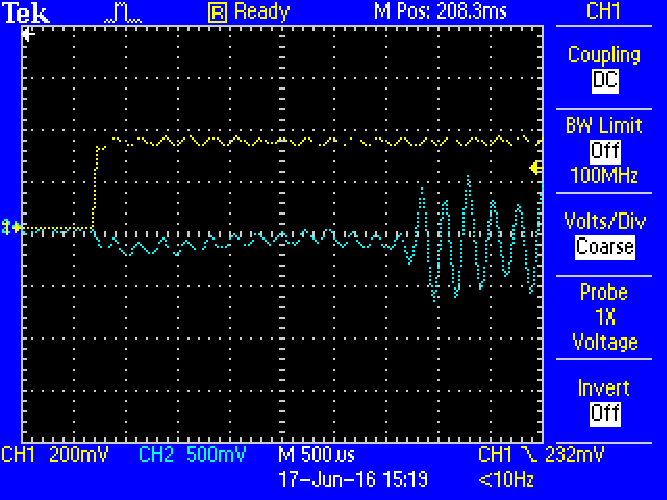
\includegraphics[width=1\textwidth]{1metersignal.pdf}
\caption{Oscilloscope measurement of the received acoustic signal at a distance of 1 meter.}
\label{1metersignal}
\end{figure}

The rising edge shows when the signal is send. The signal is then received a few moments later. Its observed that the acoustic signal arrives 3 ms later. Multiplying this with the speed of sound, a corresponding distance of roughly 1 meter was found. This supports the theory of distance measurement using acoustic signals. The received acoustic signal shows some distortion in amplitude. But the frequency is still well defined. This shows that approaches that process the received signal should be focussed on the frequency of the signal.


\subsection{Localization}
This section will cover the following subjects: Relative distance measurement, and Relative angle measurement. With these two variables the relative location of other units can be derived. 

\subsubsection{Relative distance}
Before any calculations can be done to derive the angle of other units a distance must first be determined. The first choice that has to be made is what type of signal is used to do this. The most commonly used type of signal to measure distance are radio waves, which propagate with the speed of light. Hardware to measure these  signals over short distances, would require clock-speeds of in the GHz, hence be expensive and unstable. Therefore the choice is made to use acoustic signals to measure the distance. This drastically lowers the requirements for the hardware that detects the signal.

Now that this is established there are still two ways to implement a distance measurement. These are: Time of flight (TOF)\cite{TOF}, and Received signal strength (RSSI)\cite{RSSI}. During experiments (found in section 4.3 of the Research document) it was found that the received amplitude of the acoustic signal was not proportional to the distance. It was also found that the signal was well defined over the specified distance of three meters. Because of this the signal can be detected and used for TOF.

A system is proposed that combines the two signals (radio and acoustic) in one system. Swarming modules each get their place in time to send their acoustic signal. At the moment the module starts sending the acoustic signal, it sends a message over the radio communication channel saying "I'm going to send my signal", the radio signal arrives close to instantly compared to the speed of the acoustic signal. At this point all the other modules start their timers, and stop them when the acoustic signal arrives a few moments later. The distance can now be calculated to multiply the time with the speed of sound.


\subsection{Relative angle}
Determining the relative orientation with respect to each other can be done in various ways. Some methods involved, have larger limitations than others. In general angular measurements are done using goniometric equations. It was found that calculating the angle with a single measuring point on every swarming module has one big problem\cite{Angle}. Because geometric functions are used to calculate the angle, there will always be two solutions to the equation (see figure \ref{circle} and section 3.1.1 of the Research document). To solve this the units would have to move and recalculate again to get the right answer. This would limit the units in their movement and functionality and is non-desirable.
\begin{equation}
Because\ Xp = Xq,\ cos(-\alpha) = cos(\alpha)\ applies
\end{equation}

\begin{equation}
Because\ Yq = -Yp,\ sin(-\alpha) = -sin(\alpha)\ applies
\end{equation}


To solve this problem a system is proposed with three or more acoustic receivers with a predefined distance between them. Using the difference in time and the predefined distance, the angle can be calculated with only one solution. This method is shown in figure \ref{trigonometry}.

\begin{figure}[H]
\centering
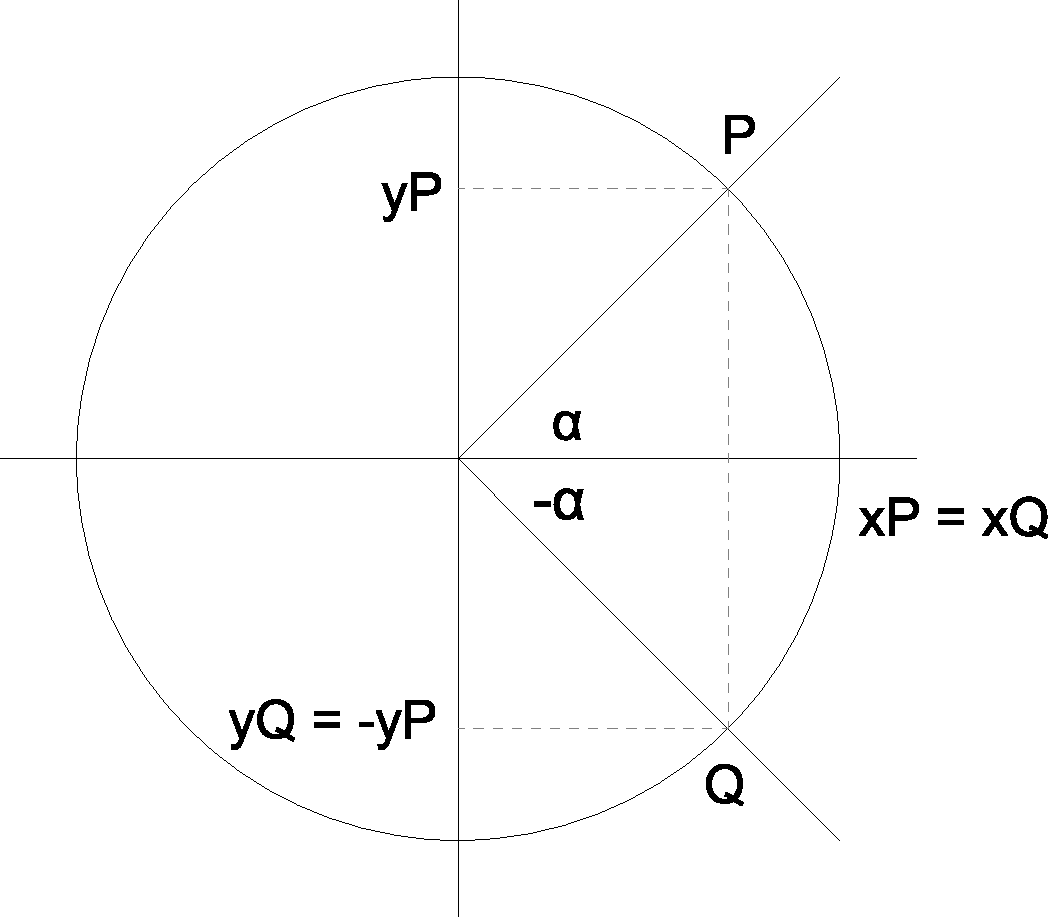
\includegraphics[width=0.7\textwidth]{Cirkel.pdf}
\caption{Unit circle where points P and Q are mirrored on the X-axes}
\label{circle}
\end{figure}



\begin{figure}[H]
\centering
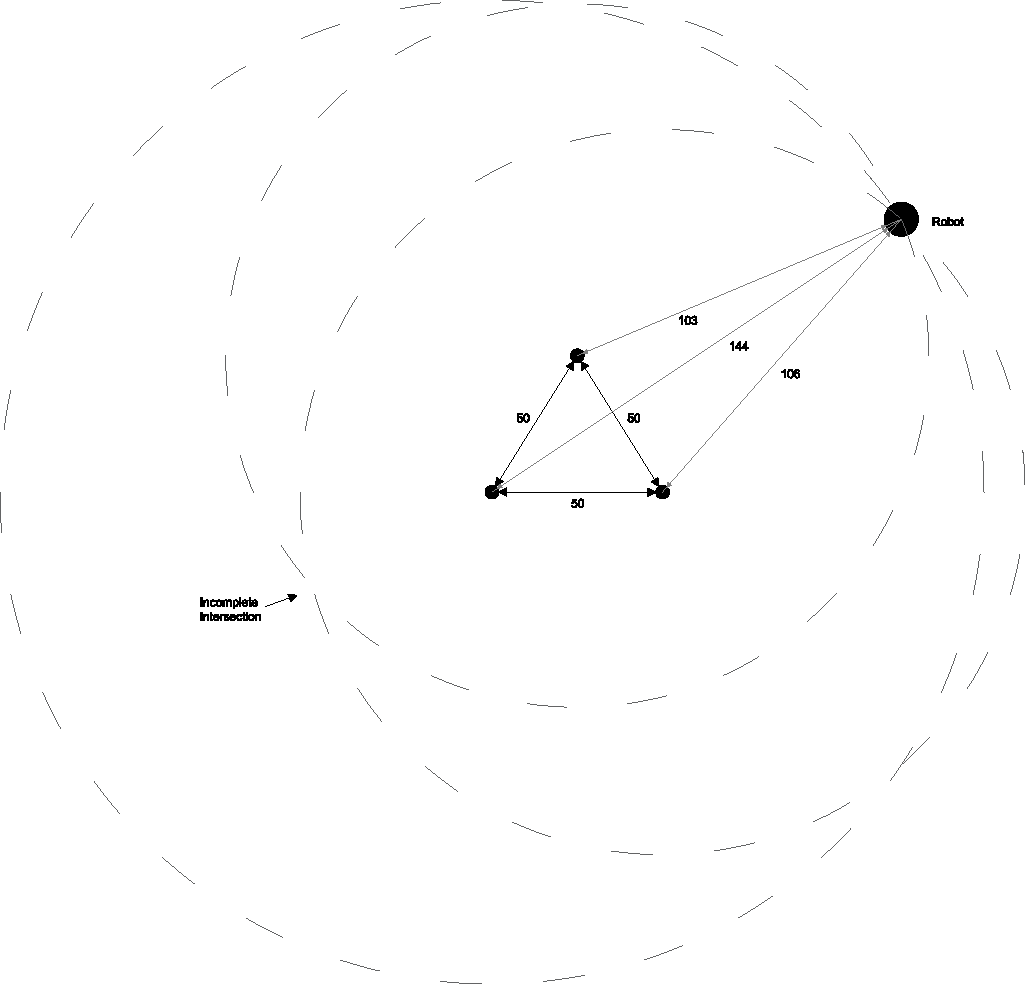
\includegraphics[width=1\textwidth]{trigonometry.pdf}
\caption{Angle determination using trigonometry}
\label{trigonometry}
\end{figure}

\subsection{Signal processing}
As talked about before the signal will be modulated and demodulated to introduce a reference point in the signal. This reference point is used to  determine the exact time the signal has travelled. Also the incoming signal from the microphone will suffer from noise and interference. Because of this the demodulator should be noise resistant. Also its part of the specification of the swarming module that it should be a robust system. Therefore the use of high clock micro-controllers and complicated software are not preferred.

Project members have experience with frequency demodulation using an analog PLL, and were confident this could be easily tested relatively quick. The PLL can be configured for high noise insensitivity using phase comparator one of the 4046CD chip, this is stated in the PLL designer guide /cite{plldisgn}. In section 9.3 of the research document it was stated that in theory, the time delay created by the PLL should be constant. This is because the delay is created by the RC time of the filter, which is a constant. A constant delay it easily compensated and will not limit the system. The PLL approach will discussed in the next section.

\subsubsection{Analog Phase locked loop}
In this experiment a 4046CD PLL is used to demodulate an acoustic signal. Time measurements are done to analyse the behaviour of the PLL, and test its potential to be used for this project. A window comparator translates the VCO-in voltage into binary code. The comparator was used instead of the ADC of the microprocessor to reduce overhead created by the sampling of the ADC. The timer on the micro-controller is now triggered by a binary '1' created by the comparator see figure \ref{fig:pllsignal}.

\begin{figure}[H]
   \centering
   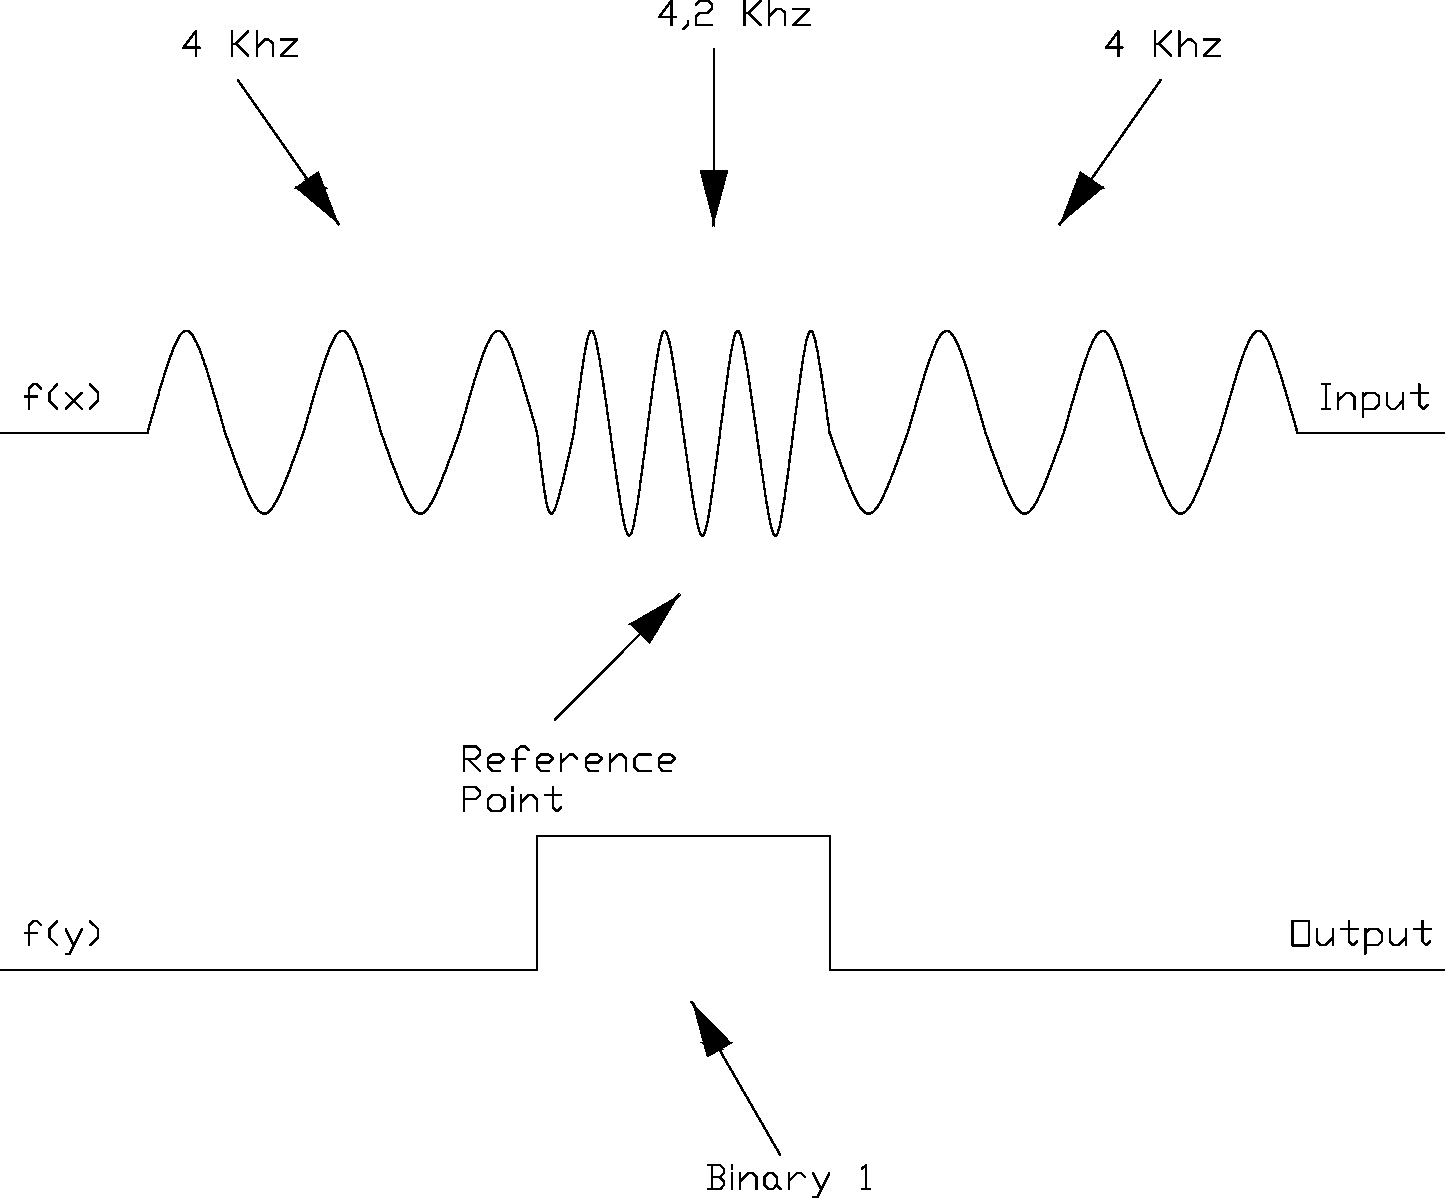
\includegraphics[width=\textwidth]{pllfsk.pdf}
   \caption{Example receiving signal PLL}
   \label{fig:pllsignal}
\end{figure}

To test the precision in time a test set-up was build. Two ATXmega128A4U were used, one for the demodulator side and one for the modulator side see figure \ref{fig:testup}. The PLL demodulator is build according to the schematic shown in figure \ref{fig:pllschematic}.

 \begin{figure}[H]
   \centering
   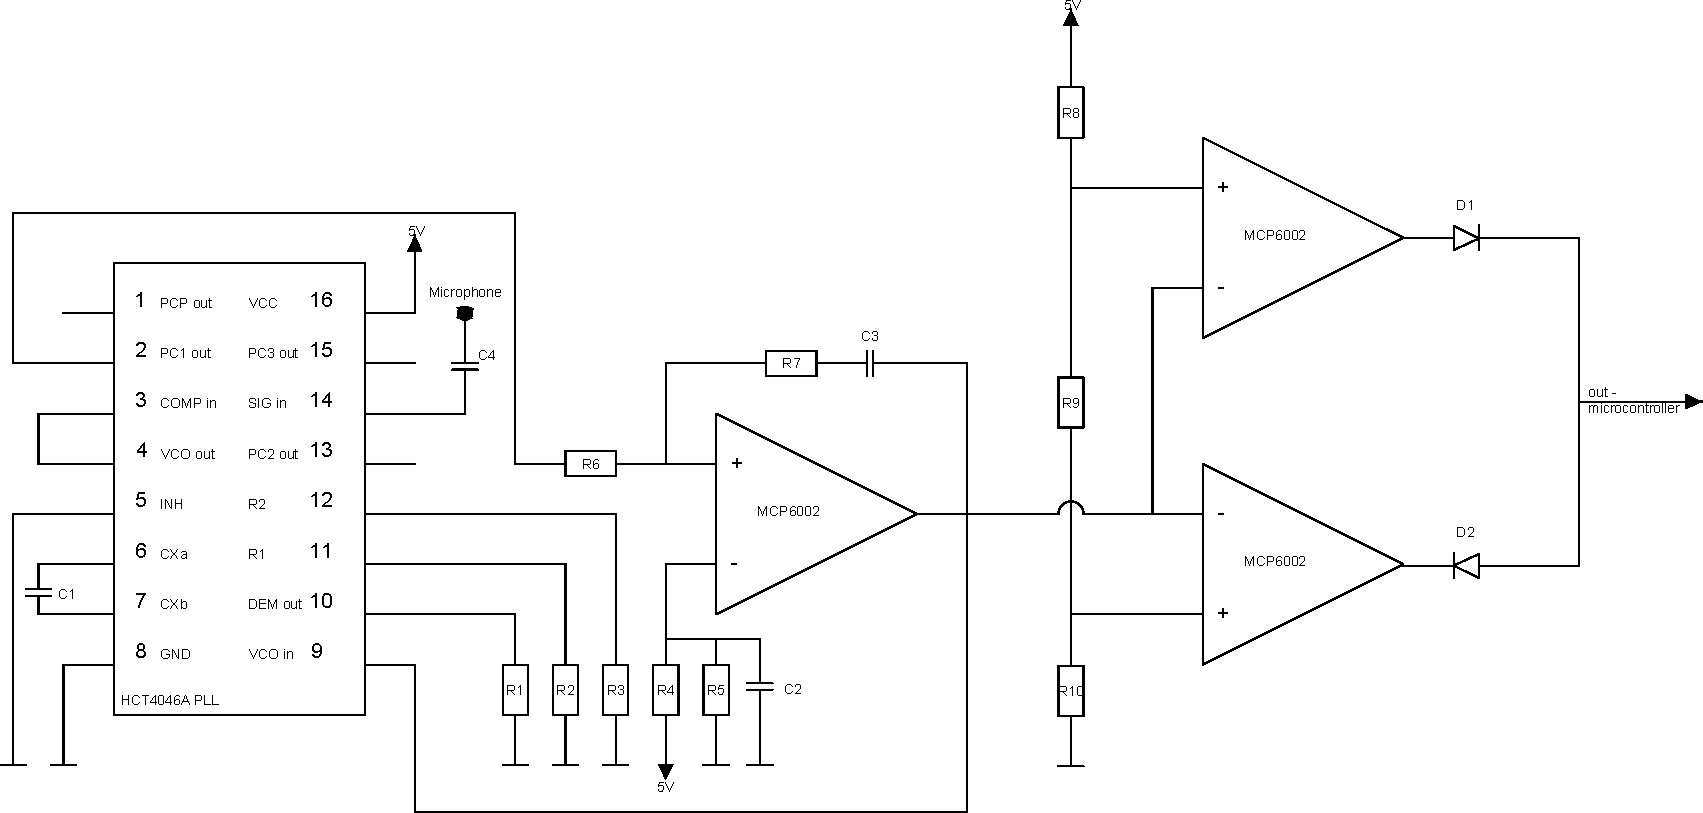
\includegraphics[width=\textwidth]{pllschema.pdf}
   \caption{PLL demodulator schematic}
   \label{fig:pllschematic}
\end{figure}

During tests the PLL was able to lock on the acoustic signal from a maximum distance of 4 meters which is well within the specification of 3 meters.  The PLL was also able to demodulate the FSK signal at this range. So now the reference point can be identified by the demodulator.

\begin{figure}[H]
   \centering
   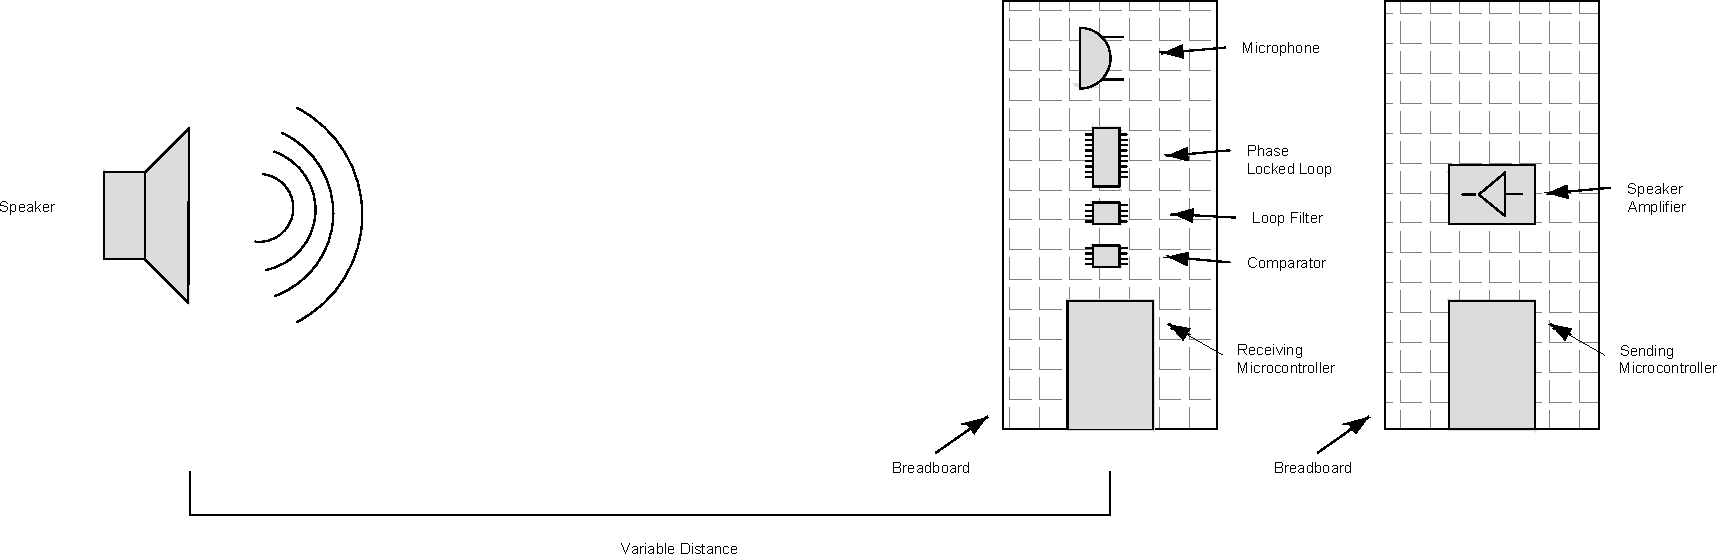
\includegraphics[width=\textwidth]{testopstellingpll.pdf}
   \caption{Test set-up demodulating with the PLL}
   \label{fig:testup}
\end{figure}

% Please add the following required packages to your document preamble:
% \usepackage{graphicx}
\begin{table}[h]
\centering
\resizebox{\textwidth}{!}{%
\begin{tabular}{|l|l|l|l|l|l|l|l|l|l|l|}
\hline
Measure point & 1       & 2       & 3       & 4       & 5       & 6       & 7       & 8       & 9       & 10      \\ \hline
0,1m        & 3115769 & 3011495 & 3048980 & 3048133 & 3113623 & 3049715 & 3112041 & 3114898 & 3041495 & 3115769 \\ \hline
1m          & 3112100 & 3012334 & 3102004 & 3159832 & 3068347 & 3123548 & 3110398 & 3119478 & 3062395 & 3119325 \\ \hline
3m          & 3130596 & 3105236 & 3120056 & 3125069 & 3140686 & 3101498 & 3130295 & 3049821 & 3101956 & 3120549 \\ \hline
\end{tabular}%
}
\caption{Measured times in clock pulses, pre scaler is set to 1 }
\label{measuretime}
\end{table}

The modulator and the demodulator are connected with a wire. The modulator sends a bit when it starts to send the acoustic signal. This bit interrupts the demodulator which starts a timer. When the reference point in the acoustic signal is detected by the PLL the window comparator sends a binary '1' to the micro-controller which stops the timer. The timer values were then printed in a terminal and are documented in table \ref{measuretime} The measured times are printed in clock pulses with a pre-scaler of 1. The test results are plotted in figure \ref{fig:testplotpll}.

\begin{figure}[H]
   \centering
   \includegraphics[width=\textwidth]{pllgrafiek.pdf}
   \caption{The test results of the PLL plotted against the expected results}
   \label{fig:testplotpll}
\end{figure}

\subsubsection{Conclusion demodulating with the PLL}
At close range the measured times seem the most stable. However some big deviations of around 500.000 clock pulses still exist. This translates in a deviations close to 5 meters, which is unacceptable. 
The digital/micro-controller side of the demodulator is tested by connecting a frequency generator to it and observing the time deviation. The time deviation was at its maximum 200 clock pulses, which is acceptable. It was observed that, when in lock the VCO-in voltage would be at a constant a stable level of 2,5V. When the frequency jump was made from 4kHz to 4,4kHz the VCO-in voltage would always rise to the same voltage of 2,78V. This means that the loop filter always has to integrate same voltage hop. The transfer function of the filter is given by equation \ref{eq:transferfunction}\cite{plldavid}.

\begin{equation}
H(p)=\frac{1+ p\tau_2}{\tau_1\tau_c(p^2+p\frac{\tau_2}{\tau1\tau2}+\frac{1}{\tau_1\tau_c})}
\label{eq:transferfunction}
\end{equation}

The transfer function shows that delays can only be caused by the time constants $\tau_1,\tau_2,\tau_3$. This eliminates the PLL-loop as the source of the deviation in delays. The comparator is the only possible source left. It was determined that the deviation in time is created by the deviation in rise and fall time of the window comparator. In conclusion it's not the PLL itself but that causes the problems but the analog to digital conversion circuit. The deviation in time observed is far too large to function as an implementation for the demodulator. The choice for not implementing the PLL with the use of an ADC was because, the only reason for implementing the PLL in analog was to enable the use of a low performance platform. Also it was observed that almost every PLL is typically used for very high frequencies up to 100 MHz and even more. Our implementation however comes close to the frequency limitation of the PLL, which could cause instability. And therefore a new method to measure time delay in the sent signal must be developed.

\subsubsection{Demodulating using the comparator of a Microprocessor}
Its been established that the analog solution does not meet the criteria. The other option is to process the signal digitally, with a microprocessor. The available micro-controller hardware during this project is Xmega based. As stated in section 5.1.1 the signal processing should be frequency based. The AVR application notes describe a straight forward way to measuring frequency using the Xemga's comparator \cite{avrfrequency}. This method is illustrated in figure \ref{fig:freqblockcount}. This method is based on counting the rising edges using the comparator, thus counting the periods. The corresponding frequency can then be derived.  

\begin{figure}[H]
   \centering
   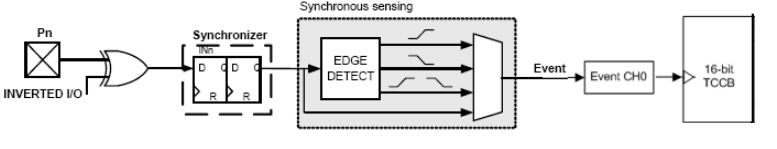
\includegraphics[width=\textwidth]{freqblockcount.jpg}
   \caption{Block representation of the frequency measurement using a Xmega \cite{avrfrequency}}
   \label{fig:freqblockcount}
\end{figure}

In the code below the measurement implementation using the comparator of the Xmega is shown. Where on line 6 to 14 an interrupt service routine is used to start the measurement and set all timers to 0. This happens when the sending unit starts sending the acoustic signal. The idea is to send a signal of 4 kHz and after a predefined amount of periods the signal stops (blank space). This blank space acts as the reference point within the signal see figure \ref{fig:acsignal}.

\begin{figure}[H]
   \centering
   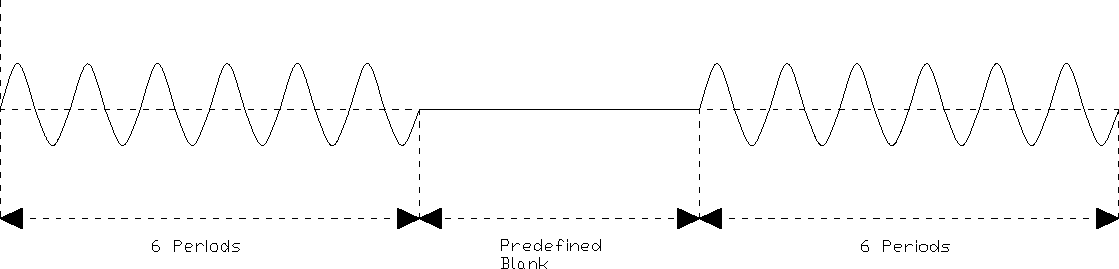
\includegraphics[width=\textwidth]{acsignal.pdf}
   \caption{Example modulated signal}
   \label{fig:acsignal}
\end{figure}


On line 22 to 38 the interrupt service routine of the comparator is used to detect every rising edge that the Xmega micro controller detects. In this interrupt the time between every edge that is detected is also measured, translating into a frequency.

On line 66 to 78 a continuous while loop has been implemented to transmit the measured frequency and the total time from the point the measurement has started till the point the measurement has stopped. The if statement checks if the frequency is of a value way below the 4 kHz and if the start-measurement flag has been set to 1, the measure value has to be equal or more than 1000 to make sure that atleast 1000 equal repeated periods have been detected.
\newpage

\lstinputlisting[firstline=1,lastline=78,label=code:codecomparator,caption=Implementation distance measurement using the Xmega comparator]{./code/comparator.c}

Tests were done at different distances, with 10 measurements at every distance, for the test set-up that has been built see figure\ref{fig:acsetup}.

\begin{figure}[H]
   \centering
   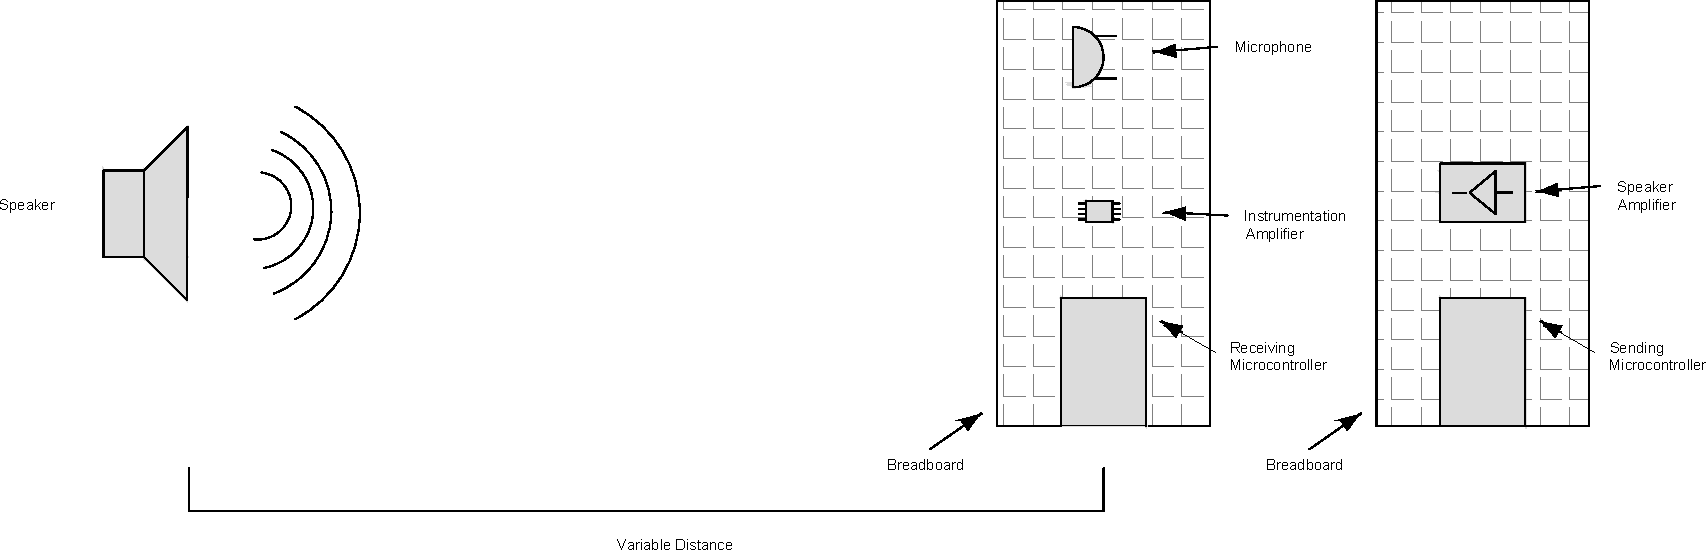
\includegraphics[width=\textwidth]{actestsetup.pdf}
   \caption{Comparator test set-up}
   \label{fig:acsetup}
\end{figure}

The measurements are plotted in a graph with the expected values are shown in figure \ref{fig:comparatorgraph}. 

\begin{figure}[H]
   \centering
   \includegraphics[width=\textwidth]{acgrafiek.pdf}
   \caption{Measured results and expected results of comparator based measurements}
   \label{fig:comparatorgraph}
\end{figure}

\subsubsection{Conclusion demodulating using the comparator}
The time delay measurement between the sent signal and the received signal gave in some circumstances promising results, however when there is just a small amount environmental noise the comparator of the Xmega picks up these sound waves disrupting the entire measurement process. No stable measurements could be accomplished using this method due to noise signals, passing through the comparators threshold generating miscounts. Due to these miscounts the large variations in measured values are generated as seen in the graph shown in figure \ref{fig:comparatorgraph}. Because of these large variations the measurements are unusable for our purpose and a new method has to be chosen. A method that is resistant to noise and is able to determine the time delay in the received signal. A more noise insensitive method called cross-correlation will be discussed in the next section.


\subsubsection{Cross-correlation}
In the previous section it was observed that digitally processing the signal showed potential. However the previous approach, suffered heavily from noise interference. Because the signal that is received is pre-defined and known a "light" version of a technique called cross correlation can be implemented. Cross correlation looks at the correlating points in the two signal arrays, the known signal and the received signal. Cross correlation has great noise insensitivity because, the noise in the received signal is uncorrelated to the signal that's already known \cite{crosscorrelation1}. 
 


\begin{equation}
R(\tau)=\int_{-\infty}^{+\infty}x(t) y(t+\tau)dt
\label{eq:Cross-correlation}
\end{equation}
\\
Where:\\
x(t) and y(t) is a function of time;\\
$\tau$ is the time delay;\\
R is the cross correlation, which is a function of the time delay $\tau$\\

Using correlation we can determine the distance as follows, consider two functions \textbf{\textit{f}} and \textbf{\textit{g}} which only differ from each other by an unknown shift along the x-axis. Using cross-correlation we can find how much \textbf{\textit{g}} must be shifted along the x-axis to make it perfectly identical to \textbf{\textit{f}}. Essentially the formula slides the function \textbf{\textit{g}} along the x-axis calculating the integral at each position. When the function are identical at each other (match), the value of \textbf{\textit{(f $\times$ g)}} is the highest number. this is because when the peaks of the signal are aligned, they make a very large contribution to the integral which should result in the highest value. 

Doing so also allows us to extract the time delay of the signal $\tau$ see figure \ref{fig:timedelay}, which in our case means the delay between sending the acoustic signal and receiving it.

\begin{figure}[H]
   \centering
   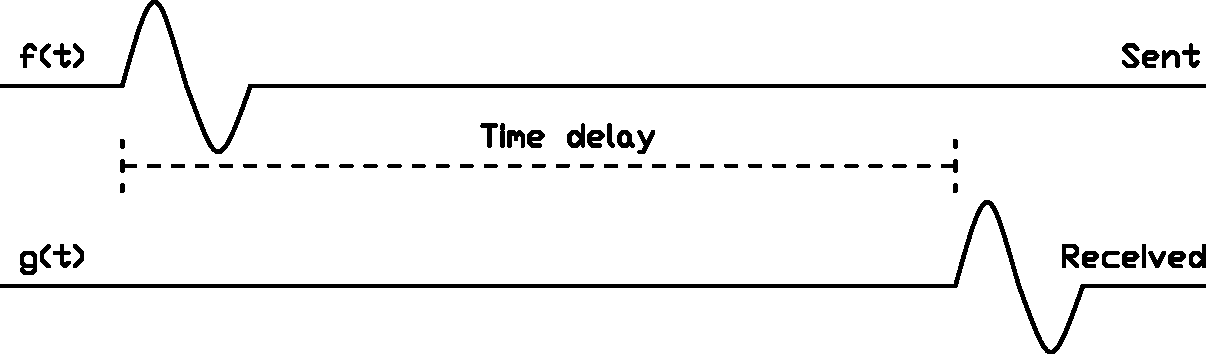
\includegraphics[width=\textwidth]{timedelay.pdf}
   \caption{Time delay between \textbf{\textit{f}} (sent) and  \textbf{\textit{g}} (received)}
   \label{fig:timedelay}
\end{figure}

As described earlier if we shift the function \textbf{\textit{g}} over the x-axis to find the point where the two signals correlate the most. Doing so the correlation process will produce several peaks. The peak where both signals correlate the most, should be the highest as shown in figure \ref{fig:correlation}. While shifting the receiving function over the x-axis it is necessary to keep track of the amount of shifts required to reach the highest point. And how many periods shifts (time shifts) required to align both signals, doing so the time delay $\tau$ can be acquired. Multiplying this with the velocity propagation of the speed of sound should give us an distance.

\begin{figure}[H]
   \centering
   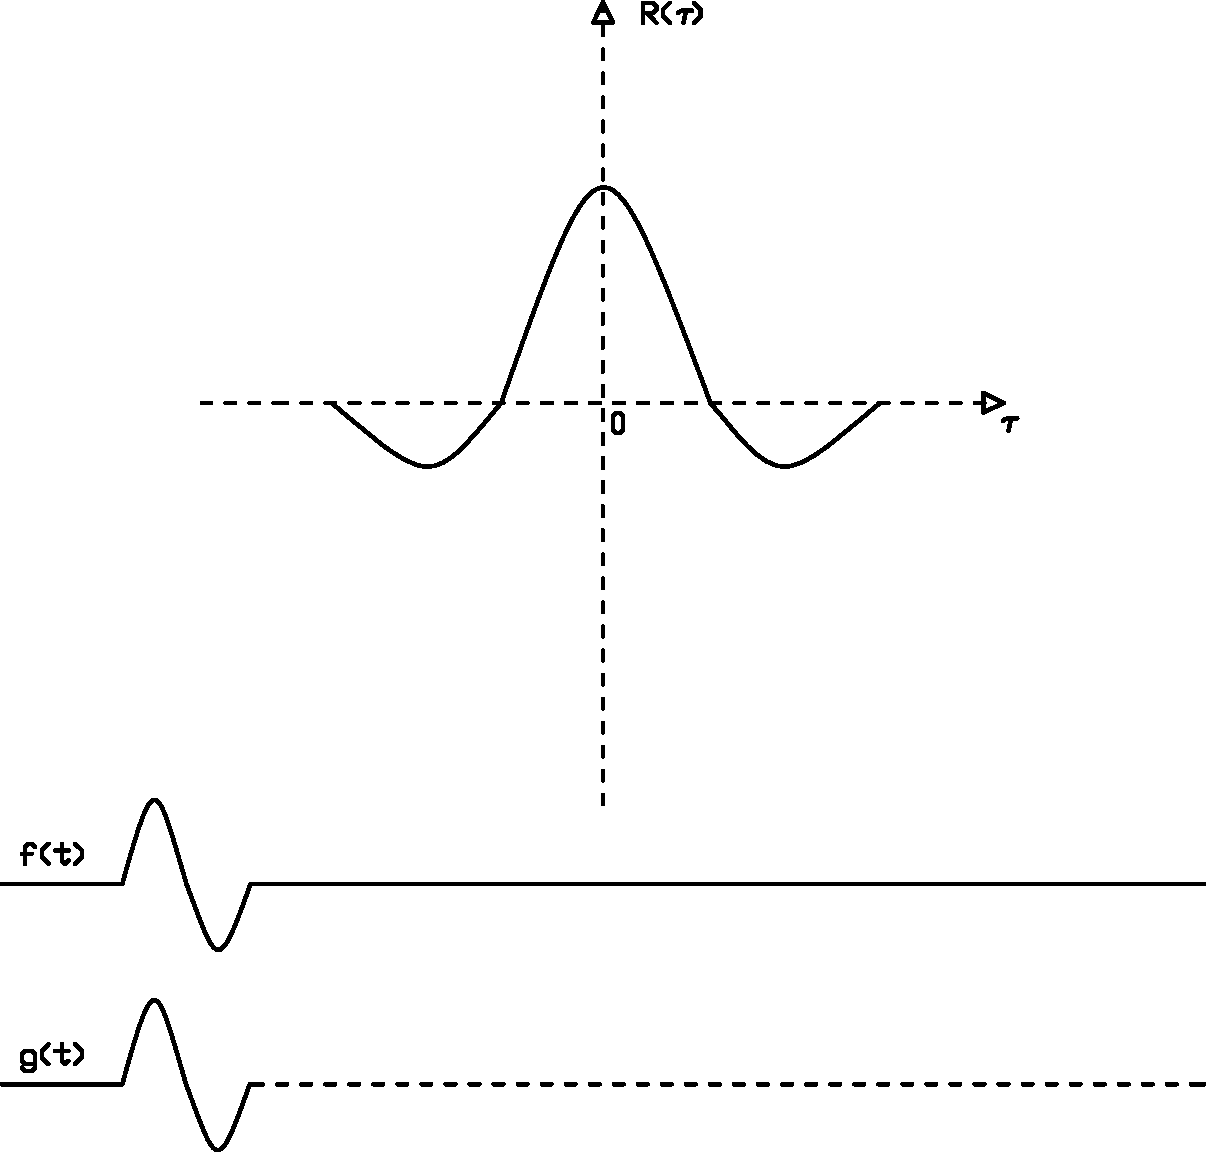
\includegraphics[width=\textwidth]{correlation.pdf}
   \caption{Auto correlation process of a cycle of a sine wave}
   \label{fig:correlation}
\end{figure}

\subsubsection{Cross-correlation implementation}
The implementation has been done in two different ways. One of them being implementing it according to the literature where a lot of floating point calculations has to be done. So we have analysed the original cross-correlation method and developed a light-weight simplified version.

This simplified has to however compromise on accuracy, but gains processing speed. Where the original cross-correlation takes up to 5 minutes in an ATXmega256A3U 32MHz Microcontroller the simplified version takes up to max 2 seconds. This increase in processing time is very crucial because when several robots move around in a swarm and it takes up to 5 minutes to generate a distance, the distance is already outdated long before it will ever be useful.

In the original cross-correlation algorithm and source code, the accuracy comes from denominator which ensures that the amplitude of the received signal has no influence on the total measurement overall. For the original cross-correlation see equation \ref{eq:correlation-formula}. The implementation of the software is shown in code 2.

\begin{equation}
R = \frac{\sum\limits_{i}^n [(x(i) - mx) * (y(i-d) - my)]}{\sqrt{\sum\limits_{i}^n (x(i) - mx)^2} * \sqrt{\sum\limits_{i}^n (y(i-d) - my)^2}}
\label{eq:correlation-formula}
\end{equation}
\\

\lstinputlisting[firstline=1,lastline=50,label=code:codecorrelation,caption=Implementation Cross-correlation]{./code/crosscorrelation.c}

\subsubsection{Simplified cross-correlation implementation}
\label{sec:simplecross}
For the simplified version of correlation where the processing time has been significantly reduced several parts of the formula has been removed. The new formula is listed below in equation \ref{eq:simplecorrelation}. The algorithm based on this formula shifts the sampled signal by one step every time till the highest value of the summation has been acquired see figure \ref{fig:simplecorrelation}. At the point where the summation gives the highest output the signals match the most. When this point has been reached the designed function implemented in c code returns the amount of shifts required in the sample array to reach this value.

\begin{equation}
R = \sum\limits_{i}^n [x(i) * y(i-d)]
\label{eq:simplecorrelation}
\end{equation}

\begin{figure}[H]
   \centering
   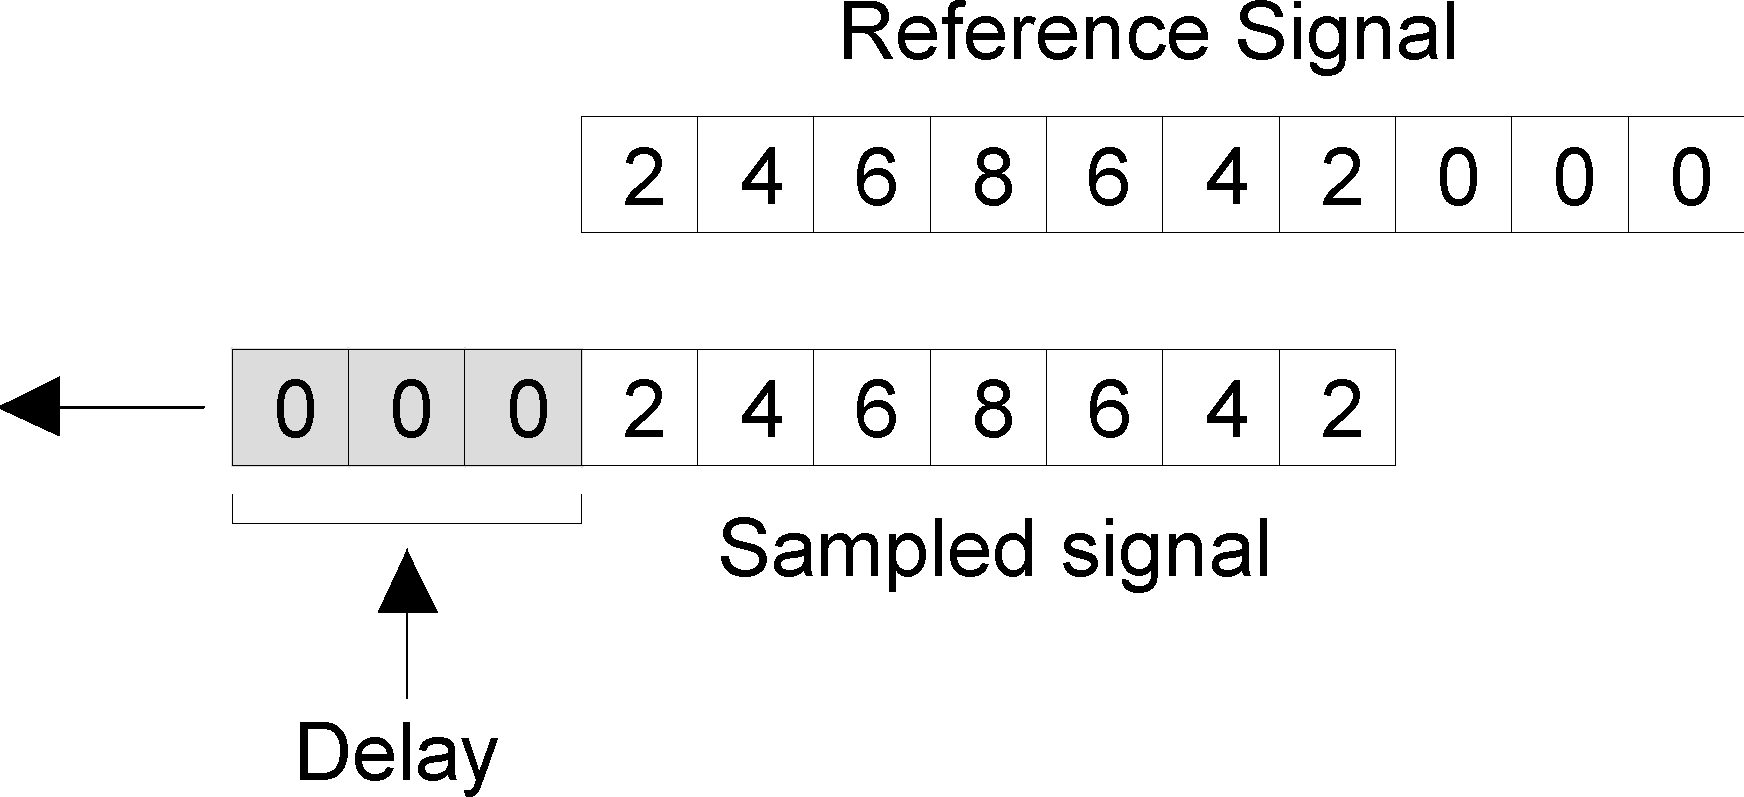
\includegraphics[width=\textwidth]{simplecorrelation.pdf}
   \caption{Algorithm simple correlation}
   \label{fig:simplecorrelation}
\end{figure}

The implementation of the source code in c is listed in below see code 3. This is a c file of the function that shifts the sampled array to align it with the reference signal. At the point where the sampled signal and the reference signal match the most the value of the time shift will be returned. And the distance can be calculated with a simple formula.
\\
\lstinputlisting[firstline=1,lastline=42,label=code:correlation,caption=Implementation Simplified version of cross-correlation]{./code/correlation.c}

\subsubsection{Cross-correlation results}
After implementing the algorithm mentioned above, several tests can be performed. With the analog to digital converter of the ATXmega256A3u the received signal from the microphone will be sampled with a sample frequency of 5\si{\micro} seconds. This means every shift that is required in the sampled array equals a delay of 5\si{\micro} seconds. With this in mind, the results we expect to see are listed in the table shown in figure \ref{fig:expectedresults}. Where the first row shows the distance, the second row shows the amount of travel time required for the distance shown in row one and the last row shows the expected shifts required. We do however expect to see some deviation in the measured results relative to the expected results due to overhead time in the processing process.

\begin{figure}[H]
   \centering
   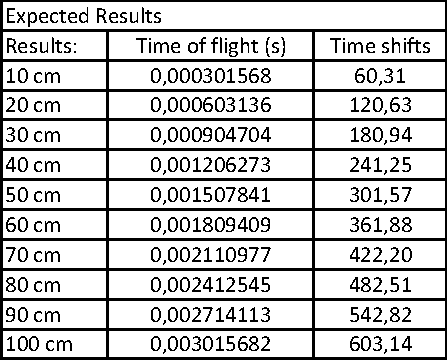
\includegraphics[width=0.45\textwidth]{expectedcorrelation.pdf}
   \caption{Expected results from the correlation algorithm}
   \label{fig:expectedresults}
\end{figure}

For the several tests that has been done the test set-up shown in figure \ref{fig:testopstelling} has been used. Where two microcontrollers, one ATXmega128A4U is used for sending the acoustic signal through the speaker and a ATXmega256A3U was used for receiving the signal with a microphone.

\begin{figure}[H]
   \centering
   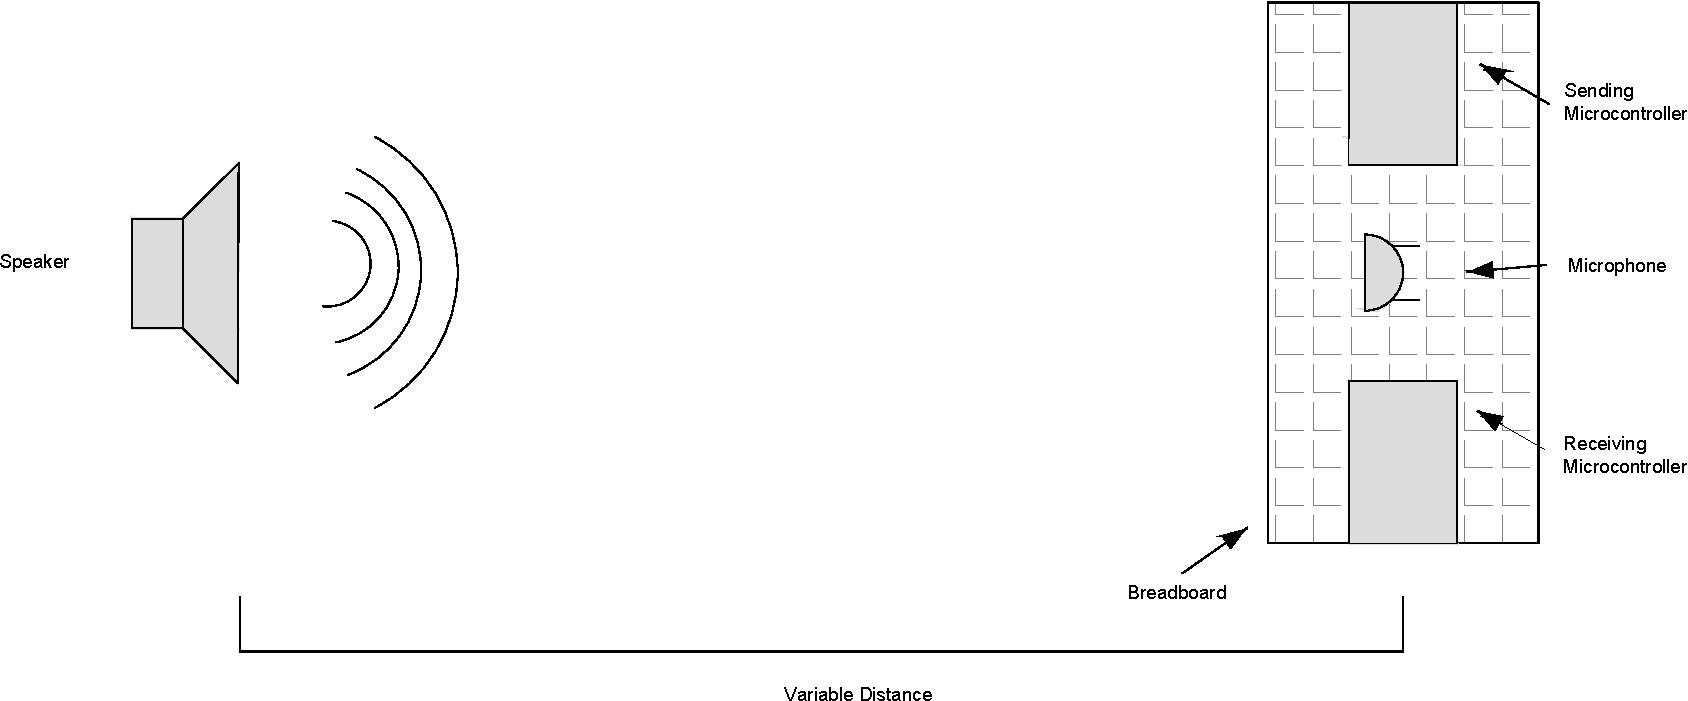
\includegraphics[width=\textwidth]{testopstelling.pdf}
   \caption{Test set-up for cross-correlation}
   \label{fig:testopstelling}
\end{figure}

In the table shown in figure \ref{fig:measuredresults} the measured results are displayed using the simplified version of cross-correlation. Per distance there are a total of seven measurements done to check for consistency in the values presented. As seen in the results at 80, 90 $\&$ 100 cm there are several faulty values measured. However most of the values measured are correct with a certain overhead time and correction.

\begin{figure}[H]
   \centering
   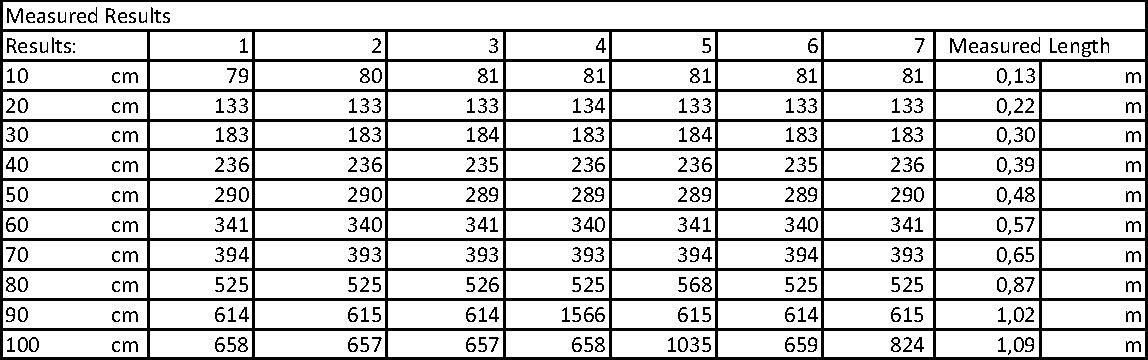
\includegraphics[width=\textwidth]{measuredcorrelation.pdf}
   \caption{Measured results from the correlation algorithm}
   \label{fig:measuredresults}
\end{figure}

In the table shown below in figure \ref{fig:deviationresults} the deviation between the expected results and the measured results are shown. As seen at close range the deviation is quite large however the further we get the more precise the measurement seems to be.   

\begin{figure}[H]
   \centering
   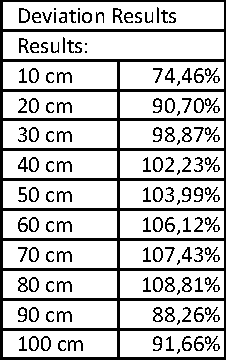
\includegraphics[width=0.22\textwidth]{deviationcorrelation.pdf}
   \caption{Deviation between measured and expected results}
   \label{fig:deviationresults}
\end{figure}

In the figure \ref{fig:grafiekcorrelation} a graph is shown with the expected values (actual distance) and the measured distance. 

\begin{figure}[H]
   \centering
   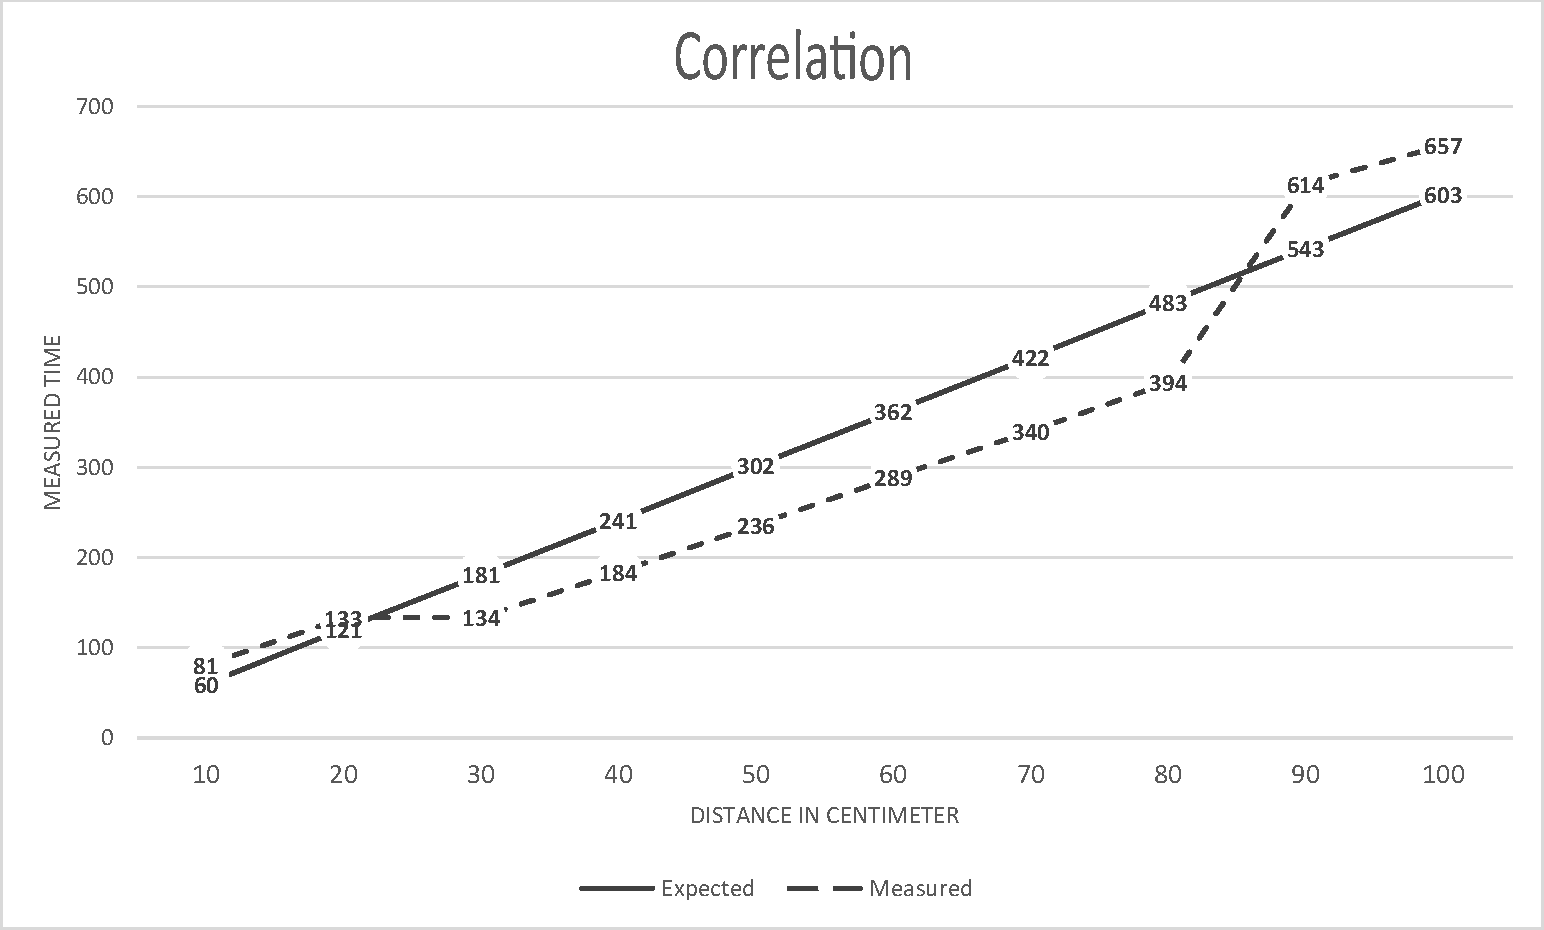
\includegraphics[width=\textwidth]{grafiekcorrelation.pdf}
   \caption{Graph of expected values versus measured values}
   \label{fig:grafiekcorrelation}
\end{figure}

However the faulty values measured still needs to be resolved because the values are in some cases very high resulting in large distances. An method to resolve this is to send multiple times and measure this signal multiple times. Doing so the histogram could be created which should display the most common values and the least common values. Choosing the most common value should increase overall stability and reduce faulty measurements.

\begin{figure}[H]
   \centering
   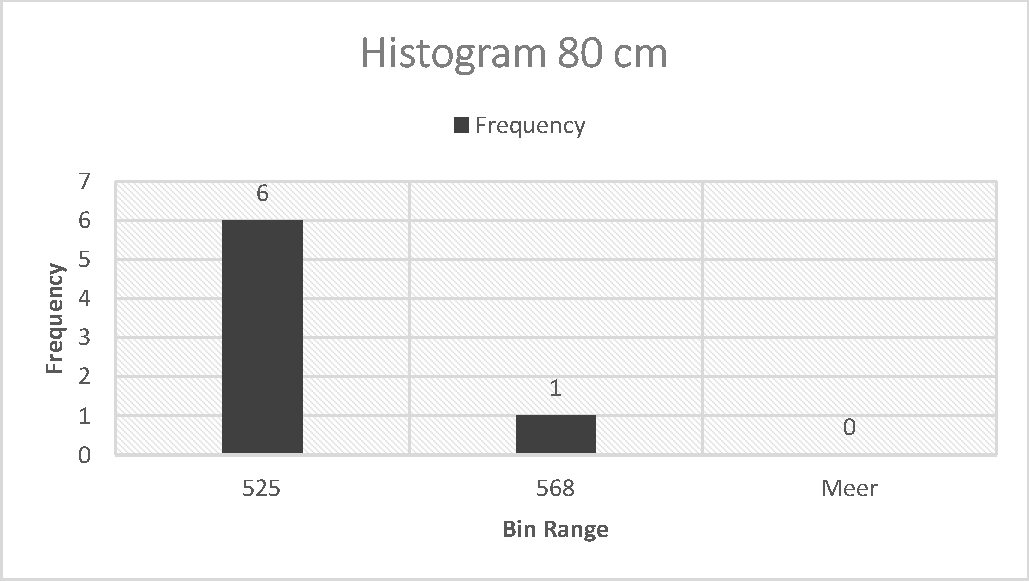
\includegraphics[width=0.82\textwidth]{histogram80.pdf}
   \caption{Histogram 80 cm measurement}
   \label{fig:histrogram80}
\end{figure}

\begin{figure}[H]
   \centering
   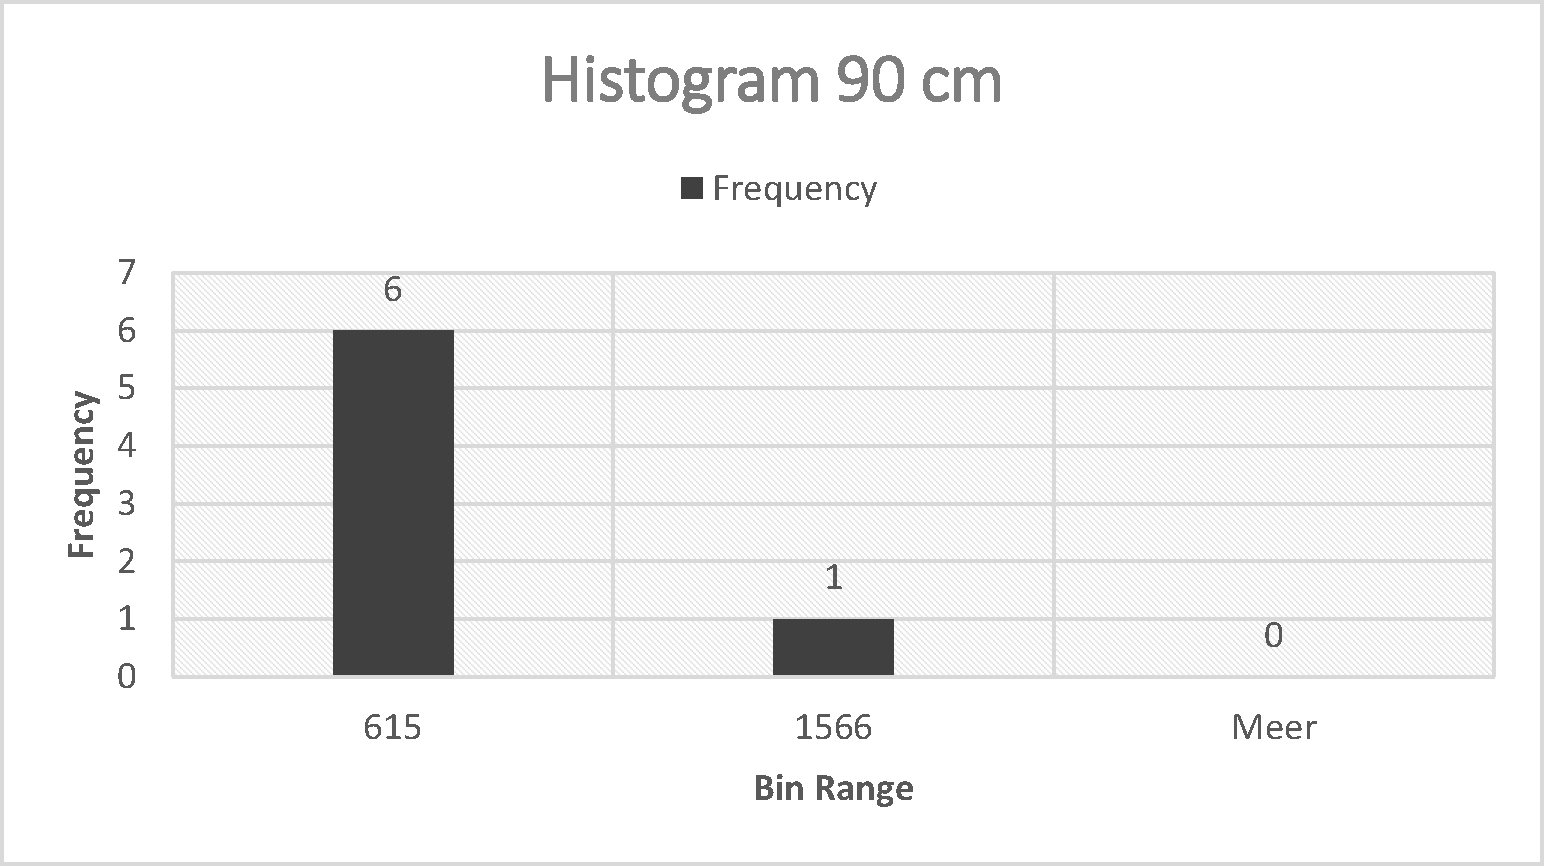
\includegraphics[width=0.82\textwidth]{histogram90.pdf}
   \caption{Histogram 90 cm measurement}
   \label{fig:histrogram90}
\end{figure}

\begin{figure}[H]
   \centering
   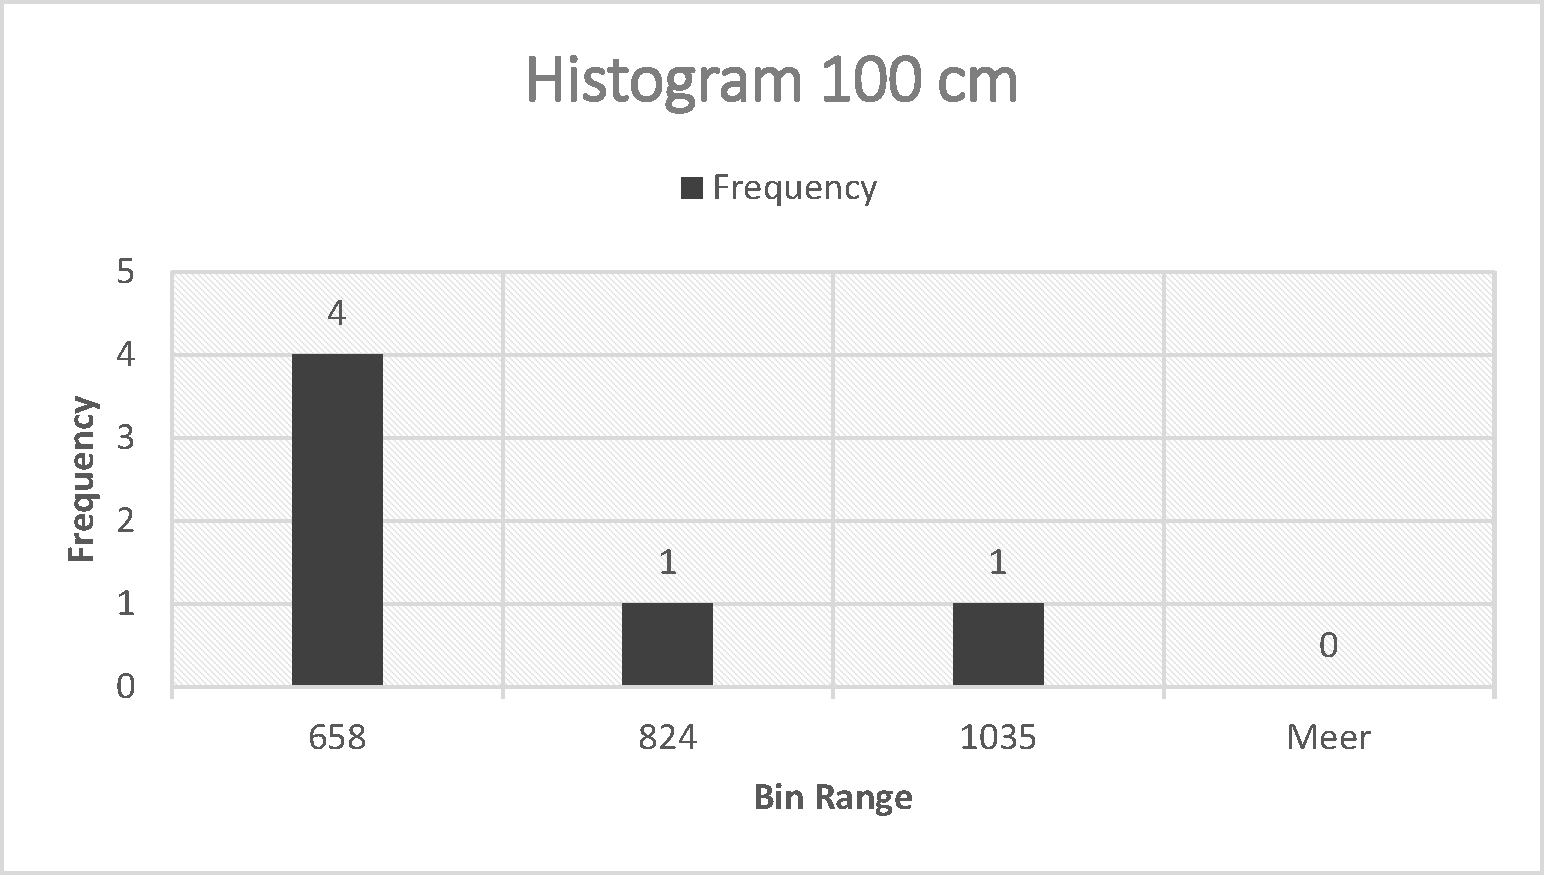
\includegraphics[width=0.82\textwidth]{histogram100.pdf}
   \caption{Histogram 100 cm measurement}
   \label{fig:histrogram100}
\end{figure}

In the figures \ref{fig:histrogram80}, \ref{fig:histrogram90} $\&$ \ref{fig:histrogram100} the histograms of the measurements with some faulty values are displayed. Implementing a method to send multiple signals and also receiving each signal independently, with the use of some filter function that chooses the most common value the output should be stable and non fluctuating. If this has been accomplished a method can be implemented to increase overall accuracy with the use of some sort of analog or digital filter that filters out other frequencies.

\subsubsection{Filtering cross-correlation}
As mentioned and showed in the results above, there is a chance that a measurement can be faulty. This could be resolved by implementing some sort of histogram filter. The idea is to receive multiple measurements and determine the most common time delay value. This is done by sending out 10 short acoustic sound signals.

At the receiving end the software determines the time delay for each acoustic signal and puts this in an array. To filter out the highest values out of the array (which are faulty), the array must first be sorted from highest to lowest value. Afterwards the two top values (highest) and one bottom value (lowest) could be removed and the rest is averaged, this algorithm is shown figure \ref{fig:filter}.

\begin{figure}[H]
   \centering
   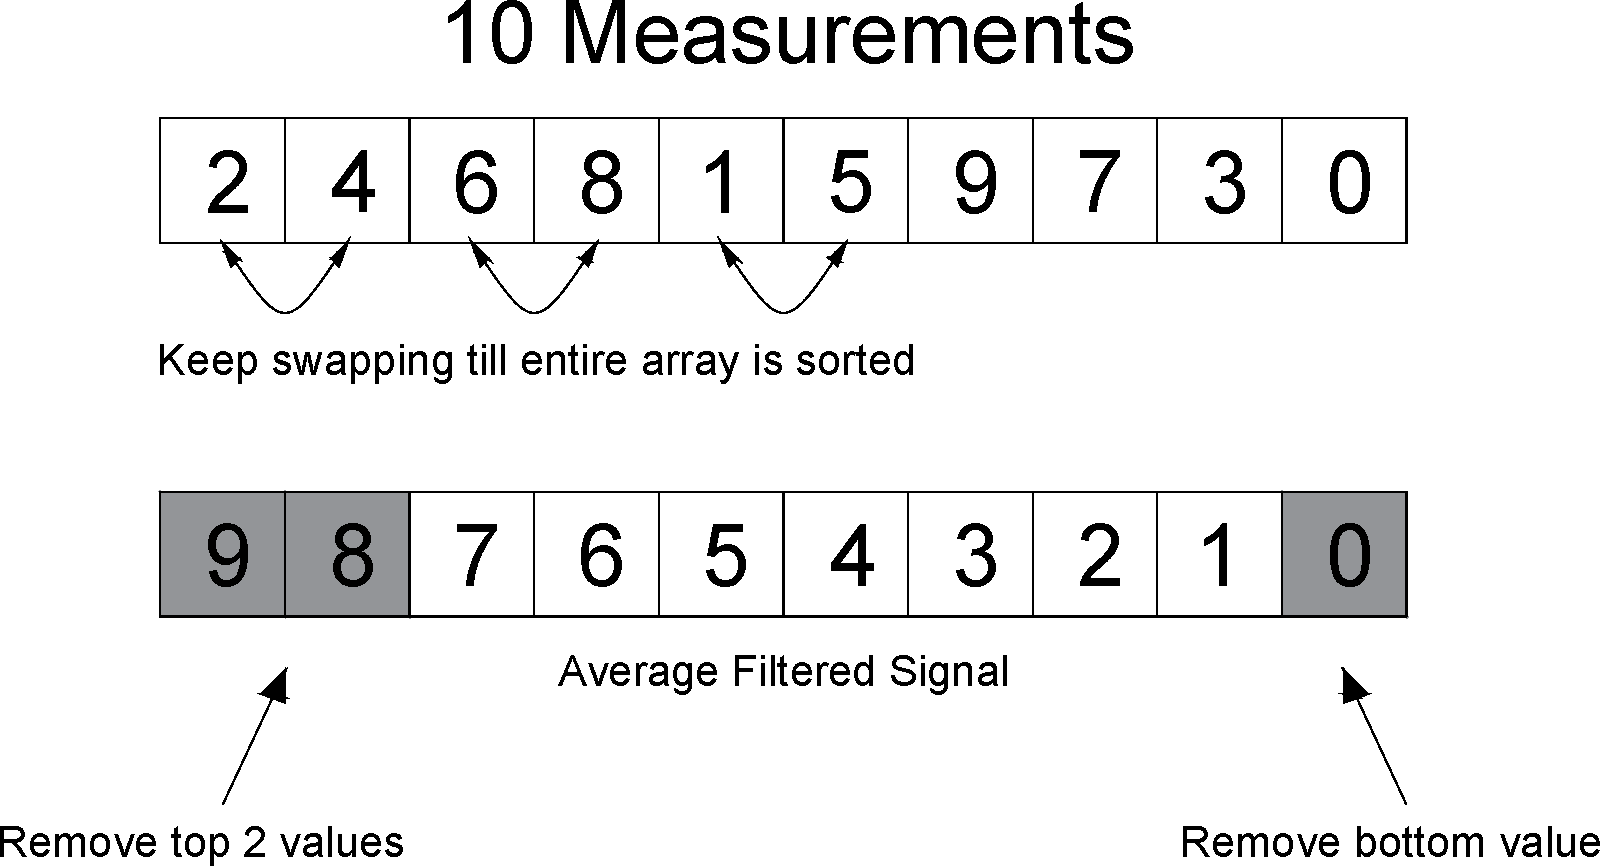
\includegraphics[width=\textwidth]{filter.pdf}
   \caption{Histogram filter algorithm}
   \label{fig:filter}
\end{figure}

This algoritm is implemented in the code 4 shown below. Where the array is sorted using the function called "Quicksort" and where the function called "Filter" removes the top two values and the bottom value and averages the leftover values in the array.
\newpage

\lstinputlisting[firstline=1,lastline=58,label=code:quicksort,caption=Implementation of histogram filter]{./code/quicksort.c}

\subsubsection{Cross-correlation results with filtering}
After implementing the filter function a new set of measurements can be taken to see how much improvement has gained from implementing such a filter. Our expectation is to atleast observe some sort of improvement towards accuracy. And also gain some distance in contrast to the previous results where only one pulse has been sent. In the table shown in figure \ref{fig:filterresults}.

\begin{figure}[H]
   \centering
   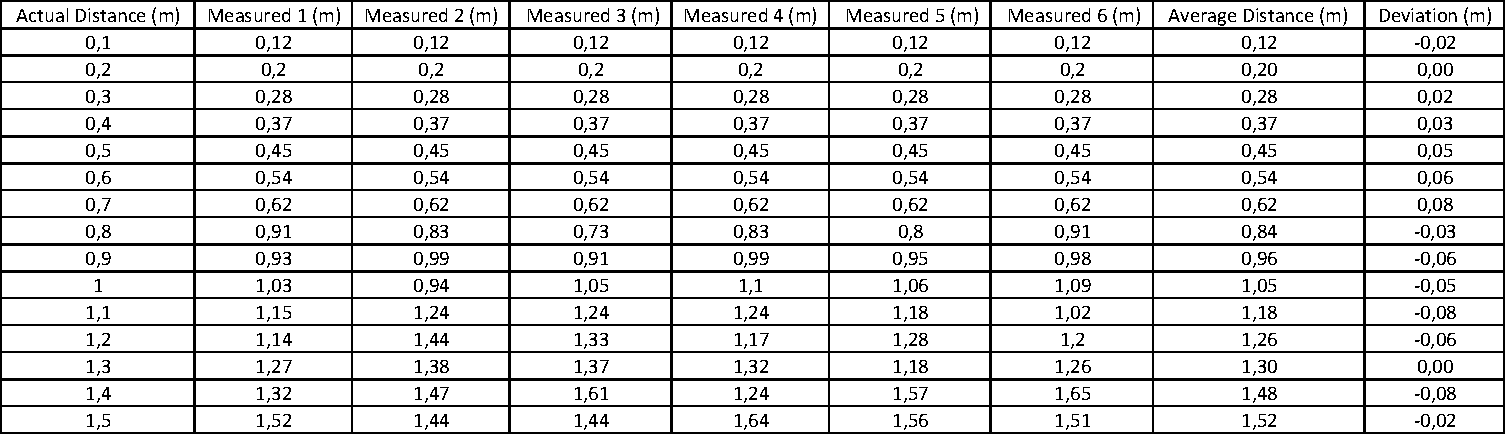
\includegraphics[width=\textwidth]{filterresult.pdf}
   \caption{Results after filtering}
   \label{fig:filterresults}
\end{figure}

As observed from the measured results shown in figure \ref{fig:filterresults}, the maximum observed deviation at this moment is +/- 0,08 meters. Whereas before the maximum observed deviation was =/- 0,12 meters, an improvement of 0,04 meters. Also an increase of 50 centimetres in gained distance has been observed whereas before only accurate measurements could be done up to 1 meter. The final results are displayed in a graph shown in figure \ref{fig:filtergraph}.

\begin{figure}[H]
   \centering
   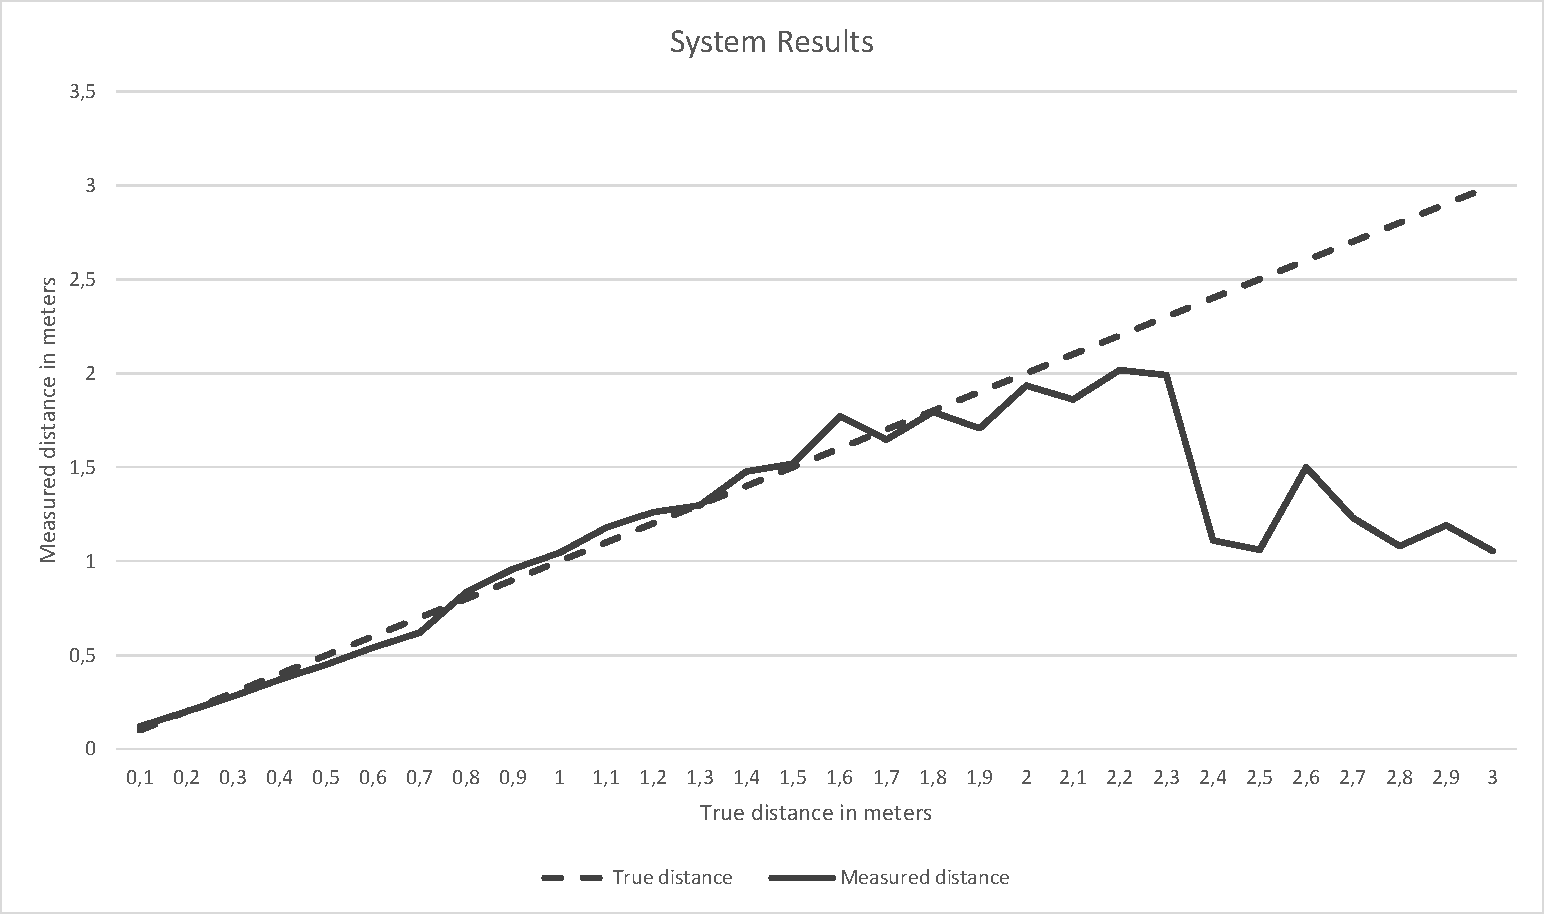
\includegraphics[width=\textwidth]{filtergraph.pdf}
   \caption{Graph of results after filtering}
   \label{fig:filtergraph}
\end{figure}

\subsubsection{Conclusion cross-correlation}
In the graph shown in figure \ref{fig:filtergraph} the expected values are set versus the measured values with the implementation of a "histogram filter" that chooses the most common value of the series of samples. 

As also seen in the graph is that the measured results do not vary as much as they did in the graph displayed in figure \ref{fig:grafiekcorrelation}, where the results did vary quite a bit relative to the expected values. 

However there is still a maximum deviation of +/- 0,08 meters observed which must be reduced to enable a localization algorithm where three microphones are used which are spread 10 centimetres apart. To overcome this a bandpass filter of some sort might increase accuracy, however at this point this is highly speculative and requires further research in this specific field. Something that could also contribute to accuracy is implementing the full cross-correlation algorithm developed by Paul Bourke instead of the lightweight cross-correlation algorithm developed and implemented by us. This implementation however needs some tweaks to dramatically increase the processing time which was as mentioned earlier up to 5 minutes with a ATXmega256A3U 32MHz microcontroller. Another approach could be to use a more powerful platform like for example a ARM Cortex processor.

Even though the results are not within the specifications (+/- 9$\%$), cross-correlation seems the be the most promising method to distinguish signals and determine the time delay. The results gathered with the implementation of a simplified version of the correlation algorithm seems to be very promising, therefore we think that an implementation of the full cross-correlation algorithm will result in stable and accurate values with some overhead time due to processing, which can be compensated for.


\subsection{Swarm communication network}
This chapter is a summarizing of chapter 'Swarm communication' in the research document of this project. The is a global research of (wireless) swarm communication networks. This research was done to determine the needed protocol(s), algorithms and the use of hardware for creating swarm networks. This chapter cites the conclusions and recommendations from the research document. Some of the important references are: \cite{combook} \cite{multi-hopwirelessnetworks} \cite{meshnetworking} \cite{position-based}.

\subsubsection{Network criteria}
There are several requirements to realise a robot swarm. Chapter 'Swarm communication' in the research document and some items in chapter 'Swarming' in this document name these requirements. 

Each member of the population needs to communicate with the rest of the swarm. A communication network is needed to make the members of the population interact with each other.

The requirements relevant for swarm communication:
\begin{itemize}
\setlength\itemsep{0em}
    \item Scalability of the swarm - It is important that the population size of the swarm is
    dynamic, because of the scalability of the swarm.
    \item Distributed communication - The use of a global channel for the coordination would influence the autonomy of the units.\cite{swarmintelligence}
    \item Wireless communication - To give the members full freedom of movement it is useful for the   communication to be wireless.
    \item Autonomy - A swarm doesn't have a master. Each member needs to be capable of maintaining the  network. These networks also must be able to reroute around nodes that have
    been lost.
\end{itemize}
Each item has additional sub criteria, this and additional information can be found in the research document.


\subsubsection{Recommendation and conclusion}
The results of the sub-study in the research document have resulted in recommendations for the implementation of the
swarming module. An enumeration of the most important recommendations is given below:
\begin{itemize}
\setlength\itemsep{0em}
    \item From all of the available network topologies, a partially connected mesh network satisfies the desired network requirements.
    \item With the use of routing protocols the network can be rerouted around nodes that have been lost. The most suitable protocol for re-routing in this situation is greedy routing or simular.
    \item Wireless communication is not only useful, it must be a requirement. Due to the mobility of the swarm members, wired communication is feasible.
    \item As stated in the research, UWB, Wi-Fi and ZigBee protocols are all suitable to create a wireless mesh swarm network. Six potential protocols have been investigated and eventually four of them are compared in the conclusion. The comparison is based on transmitting range, scalability, data coding efficiency, protocol complexity, data distribution per square meter and power consumption. The results from the comparison of the protocols don't differ much from each other, only Bluetooth stands out.
\end{itemize}
The other additional recommendations and conclusions can be found in the research document.




\section{Specifications}
Before the features of the Swarming module are specified, swarming itself should be specified further. This discussed in section 1 of the research document. By creating a set of realistic scenarios. From this specifications like: minimal distance, maximal distance, maximum number of units, and precision are derived. These specifications are summarised in Table \ref{smrange} and Table \ref{specunits}. 

\begin{table}[h]
\centering
\resizebox{\textwidth}{!}{%
\begin{tabular}{|l|l|l|}
\hline
                     & \textbf{Close range (0 - 3 m)} & \textbf{Long range (3 - 25 m)} \\ \hline
Dead zone distance    & 0,015 meters                   & 2 meters                      \\ \hline
Deviation (distance) & +/- 9\%                         & +/- 1 meter                   \\ \hline
Angle Resolution     & 45\%                            & -                             \\ \hline
Update frequency     & 40 Hz                           & 1 Hz                           \\ \hline
\end{tabular}%
}
\caption{Swarming localization specifications}
\label{smrange}
\end{table}

\begin{table}[h]
\centering
\resizebox{\textwidth}{!}{%
\begin{tabular}{|l|l|l|l|l|}
\hline
 & \textbf{minimum} & \textbf{maximum} & \textbf{maximum (close range)} & \textbf{Preferred (demonstration)} \\ \hline
Number of Units & \multicolumn{1}{c|}{3} & \multicolumn{1}{c|}{$\infty$} & \multicolumn{1}{c|}{130} & \multicolumn{1}{c|}{6 to 12} \\ \hline
\end{tabular}%
}
\caption{Specifications number of units}
\label{specunits}
\end{table}


The choice is made to divide the the specifications for localization into two categories: Close range, and long range. This choice was made because at close range more precision precision is needed to prevent the robots from crashing into each other. While at long range the localization will be used not to loose the swarm. The maximum number at close range is derived from the theoretical number of units that can physically fit in a 3 meter radius. And the preferred number of units for demonstration purpose is used to set a goal for the project. For further clarification how these specifications are determined see chapter one of the research document.



\subsection{Wireless communication}

In Table \ref{wcm} a more detailed version of the specifications are written down. From these specifications the module will be implemented as is shown in the next section. 

\begin{table}[H]
\centering
\caption{Wireless communication module}
\label{wcm}
\begin{tabular}{|p{1,5cm}|p{9,5cm}|}
\hline
Module   & Wireless communication module                                       \\ \hline
Input    & 5 VDC\\ 
        & Swarm data\\
        & RF signal                                              \\ \hline
Outputs  & RF signal                                           \\ 
& Swarm data \\ \hline
Function & Processes information to and from other swarm modules. Transmission speed is not defined yet. The transmission range must be around 100 meters or more. \\ \hline
\end{tabular}
\end{table}
\subsection{Central operating unit}
The central operating unit processes data from the sensors and swarm network. This unit uses the external wireless swarm communication, the local communication bus and the debug interface as an communication channel. The local communication bus uses a TWI (Two Wire Interface) protocol and is used for the communication with the robots peripherals i.e. actuators. The debug interface of the central operating unit uses an UART protocol to communicate with external systems for debug purposes.

\begin{table}[H]
\centering
\caption{Central operating unit}
\label{cou}
\begin{tabular}{|p{1,5cm}|p{9,5cm}|}
\hline
Module   & Central operating unit                                        \\ \hline
Input    & 3,3 VDC \\
         & Data streams (TWI, UART)                                           \\ \hline
Outputs  & Data streams (TWI, UART)                                             \\ \hline
Function & Calculates the relative position to other swarming modules. Distributes local and external data streams. Analyses and uses sensor information.\\ \hline
\end{tabular}
\end{table}


\section{Functional specification}
This chapter describes the functional design of the swarming module. An overview of the swarming module is given in figure \ref{overall}. The module is designed in such a way that it is modular. This module can be placed on an object (i.e. a robot) and can be used by the object to send and receive relevant information about other in-range swarming modules.\\

This chapter discusses the following subjects:
\begin{itemize}
\setlength\itemsep{0em}
\item Swarming module
\item Power supply and safety
\item Central operating unit
\item Wireless communication module
\item Relative orientation sensor
\item Orientation sensor
\item Localisation sensor
\end{itemize}

\subsection{Swarming module}
The overall design of the swarming module is shown in figure \ref{overall}. Each block of the overall design is described in the following figures. The central operating unit is at the hearth off the swarming module, and takes care of the localization algorithm.
\begin{figure}[h]
  \centering
      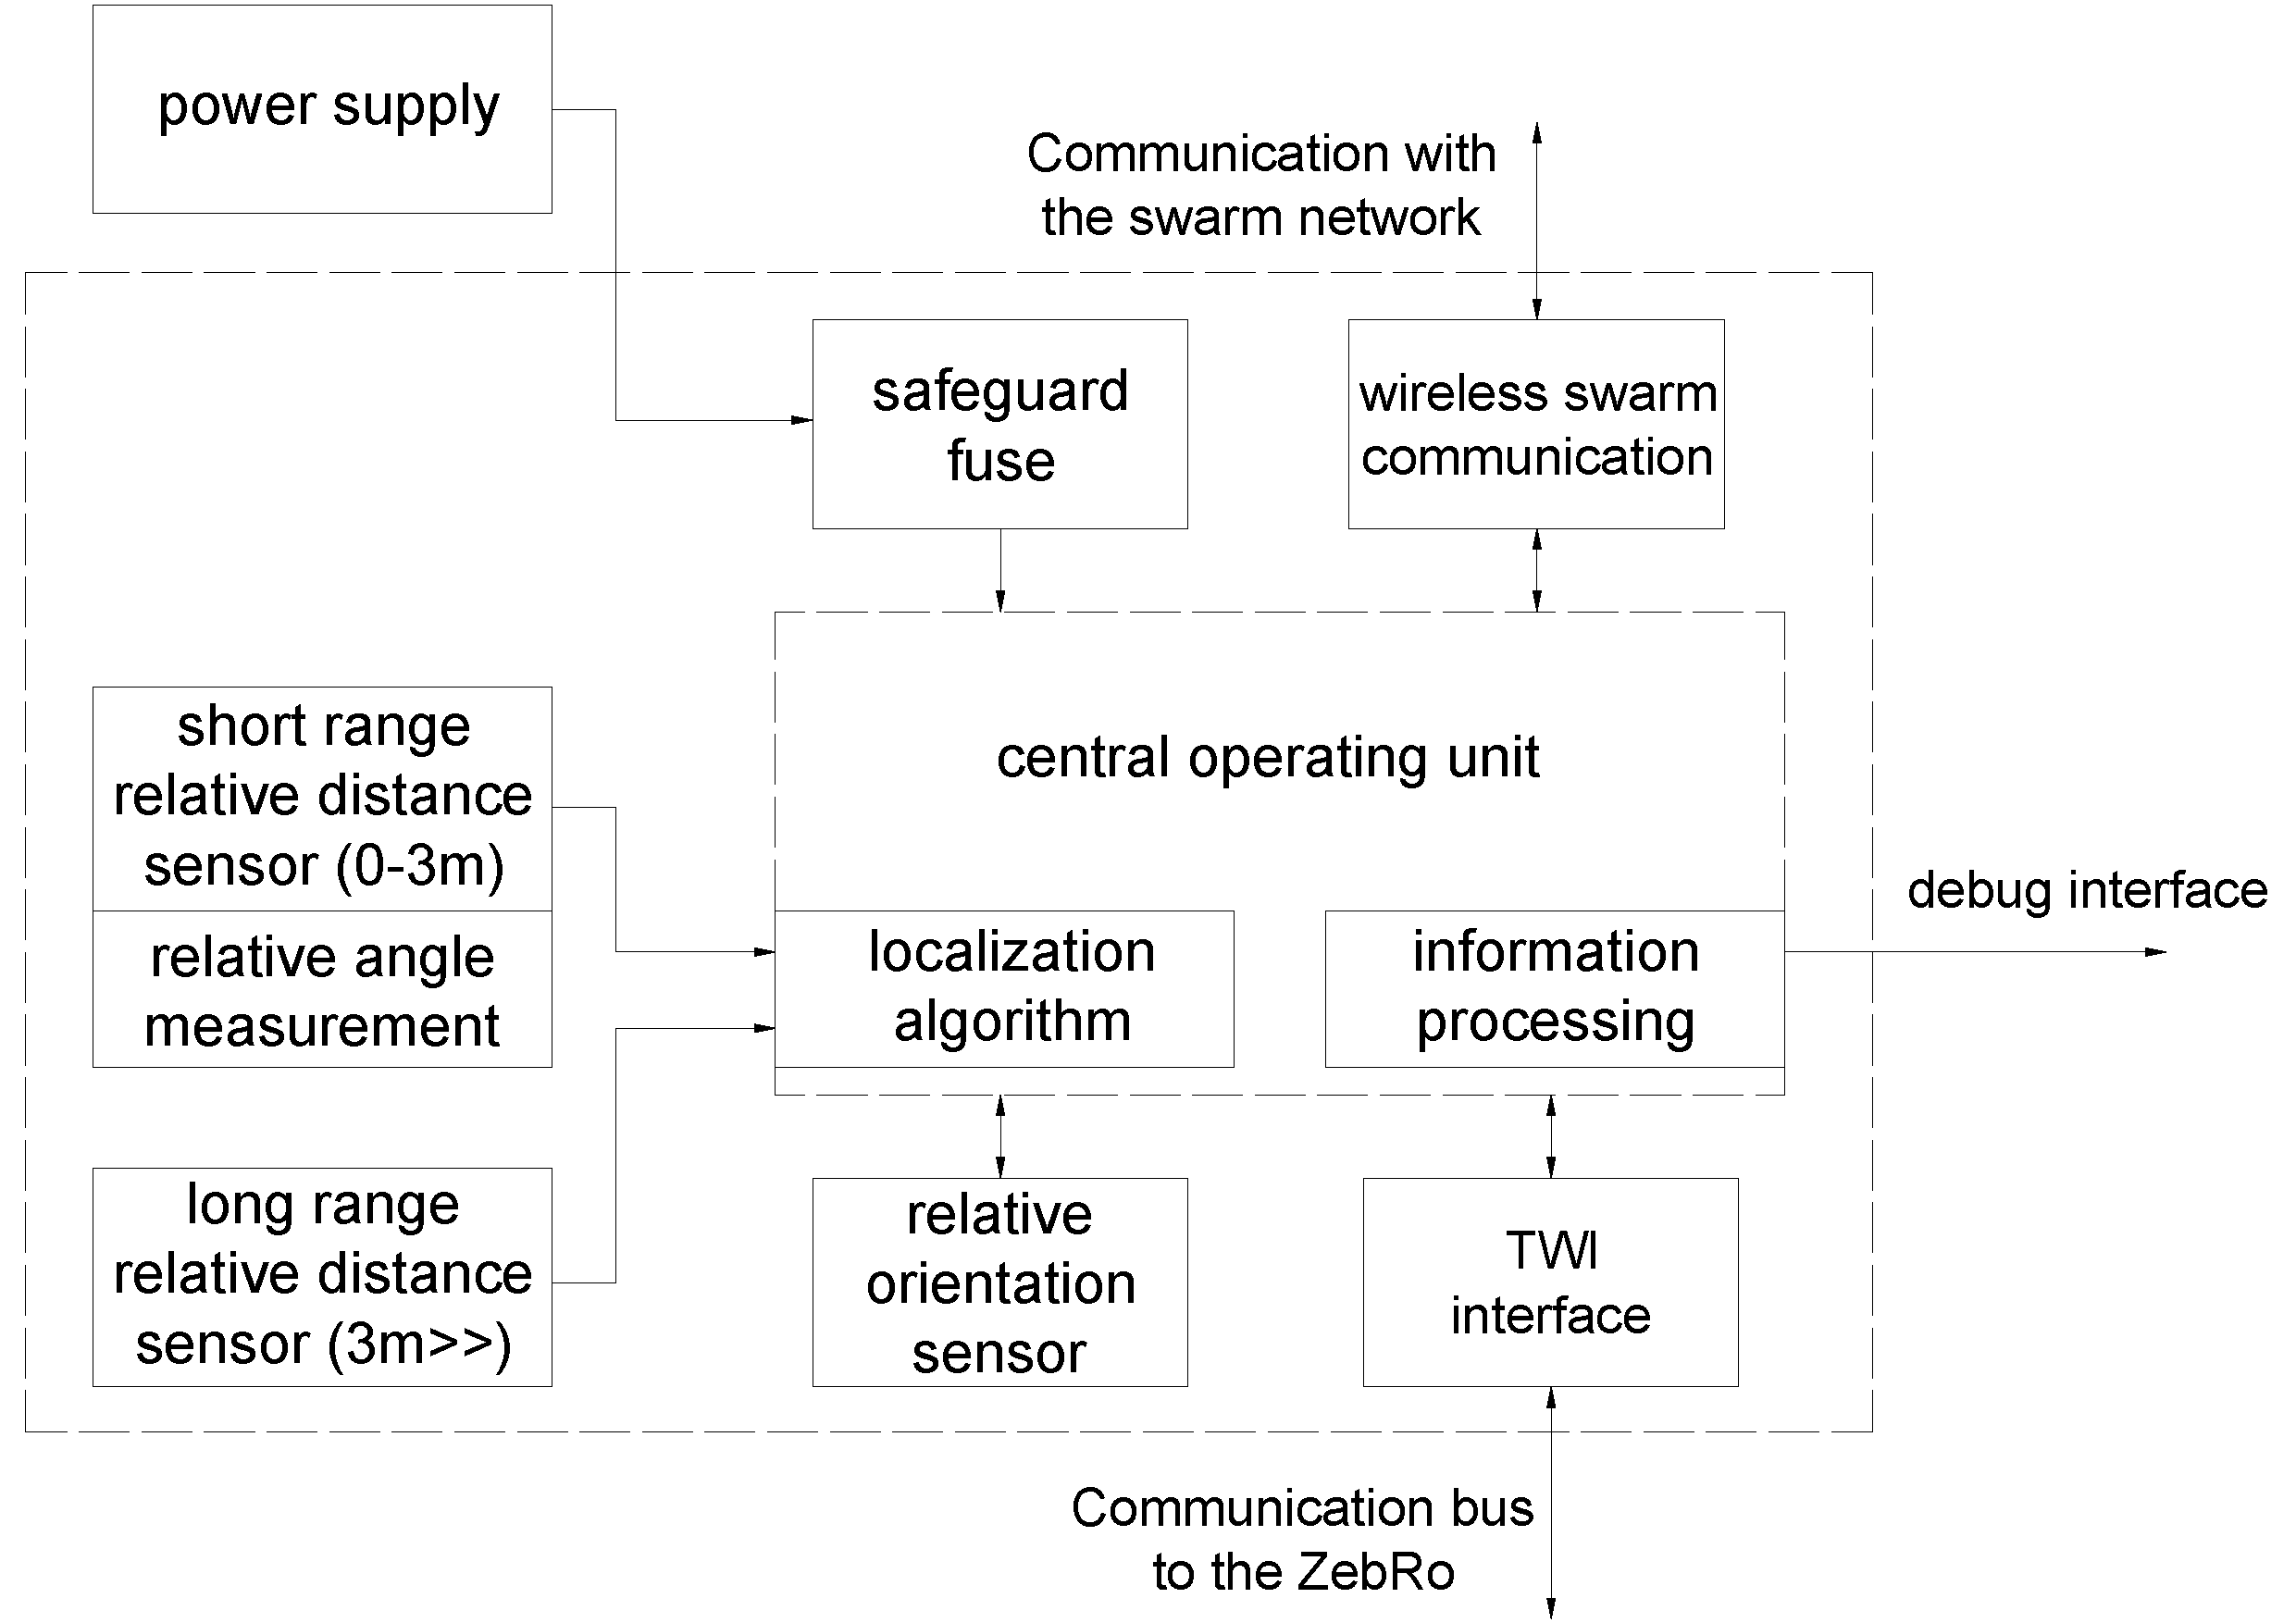
\includegraphics[width=1\textwidth]{overall.pdf}
  \caption{Overview of the swarm module design}
  \label{overall}
\end{figure}

\subsection{Short range localisation sensor}
The principle of the short range localisation sensor is displayed in figure \ref{demodulator} and \ref{modulator}. As mentioned earlier the short relative distance measurement will be done acoustically. With acoustic sensing it is required to let the speaker sway to the right oscillation frequency, reaching this oscillation frequency takes time since the speaker won't oscillate at the right frequency instantly. This complicates the measurement a little bit, since just detecting the to be measured signal won't always translate into an exact distance due to the time the speakers take to sway into oscillation.

A solution to this problem is to create a fixed reference point within the sent signal. Creating this reference point after a fixed time enables the speaker to sway into oscillation making sure that no faulty measurements occur do to this “swaying time”. When the reference point has been detected by the receiver an accurate distance can be determined by subtracting the fixed “sway time”.

Without the implementation of this fixed reference point it is possible for a receiver to miss a few periods of the signal, due to the speaker still swaying into oscillation and the time of swaying being unknown. For example take an acoustic signal (Speed of sound 340.29 m/s) with a frequency of 4000Hz, one period of this signal is 0.00025s. Missing one period of this signal translates into a distance error of 8.5cm. Since the sway time of a speaker can change over time due to mechanical stresses a fixed time stamp seems the most suitable solution for the long term. The best way to create this reference point it still to be determined. This will be done by either frequency shift keying or phase shift modulation. Some real like testing will have to determine the best method.

\subsubsection{Modulation}
The modulation method is going to be determined by how well the reference point can be recognized by the demodulator. In the research phase, test were done with an speaker and a microphone. This showed that frequency and phase were well defined over distance but amplitude was not. Because of this the available methods for modulation of the acoustic signal are frequency modulation or phase modulation. The most important feature of the modulator must be consistency, meaning that the reference point should be send at exactly the same point in the signal every time. This is so that no deviation will occur when compensating for the missed periods before the reference point. In theory this can be done by both of the methods. 


See figure \ref{modulator} for a schematic representation of the modulator.

\begin{figure}[H]
  \centering
      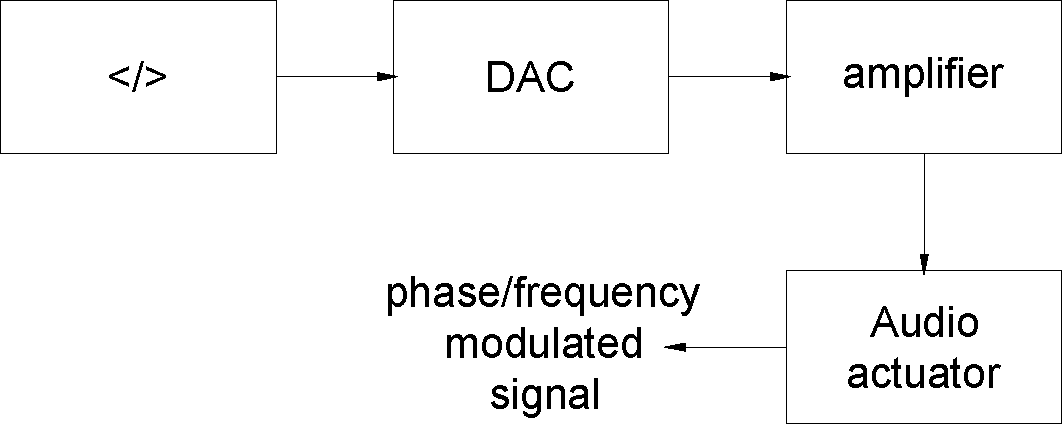
\includegraphics[width=0.8\textwidth]{modulator2.pdf}
  \caption{Modulator}
  \label{modulator}
\end{figure}

\subsubsection{Demodulation}

A demodulator will be needed to retrieve the digital signal send from one swarm-module to another.  One swarming module will send an acoustic signal to the other modules, this signal will then be picked up by an sensor and will need to be processed properly before it can be used to determine the time it took the acoustic signal to travel from one swarming-module to the other. The signal retrieved by the acoustic sensor will also pick up a lot of noise and other sounds from the environment. Also, when further away the signal might be low in amplitude. To increase the amplitude and lower the noise, the signal will be amplified and filtered. These modifications to the signal will improve the signal to noise ratio drastically but a lot of noise might still remain. Therefore the demodulator itself must be insensitive to noise.  
The main purpose is the demodulator is to identify the reference point. And more importantly, determine the point in time the reference point is spotted. The time determined will be used to calculate the distance. Hence, the precision in which the demodulator determines the reference point in time effects the precision of the distance measurement. Only one swarming module will be sending his acoustic signal at any moment. When there are 10 units in its specified range and a preferred update frequency of 40Hz (see section 1). This gives every swarming-module only a small window in time to send their signal and for the other to receive it. When a frequency of 4kHz is chosen for the signal, every swarming-module will have 10 periods to send their signal. There for the demodulator must be able to lock onto the signal and determine the reference point within a few periods of the acoustic signal. See figure \ref{demodulator} for a schematic representation of the demodulator.

\begin{table}[H]
\centering
\caption{Demodulation specifications}
\label{demosensor}
\begin{tabular}{|p{1,5cm}|p{9,5cm}|}
\hline
Module   & Demodulator                                   \\ \hline
Input    & FSK Signal                                             \\ \hline
Outputs  & Reference point                                         \\ \hline
Function & Demodulation, Reference point detection \\ \hline
Features & Noise insensitive, precision (time), Quick demodulation  \\ \hline
\end{tabular}
\end{table}

\begin{figure}[H]
  \centering
      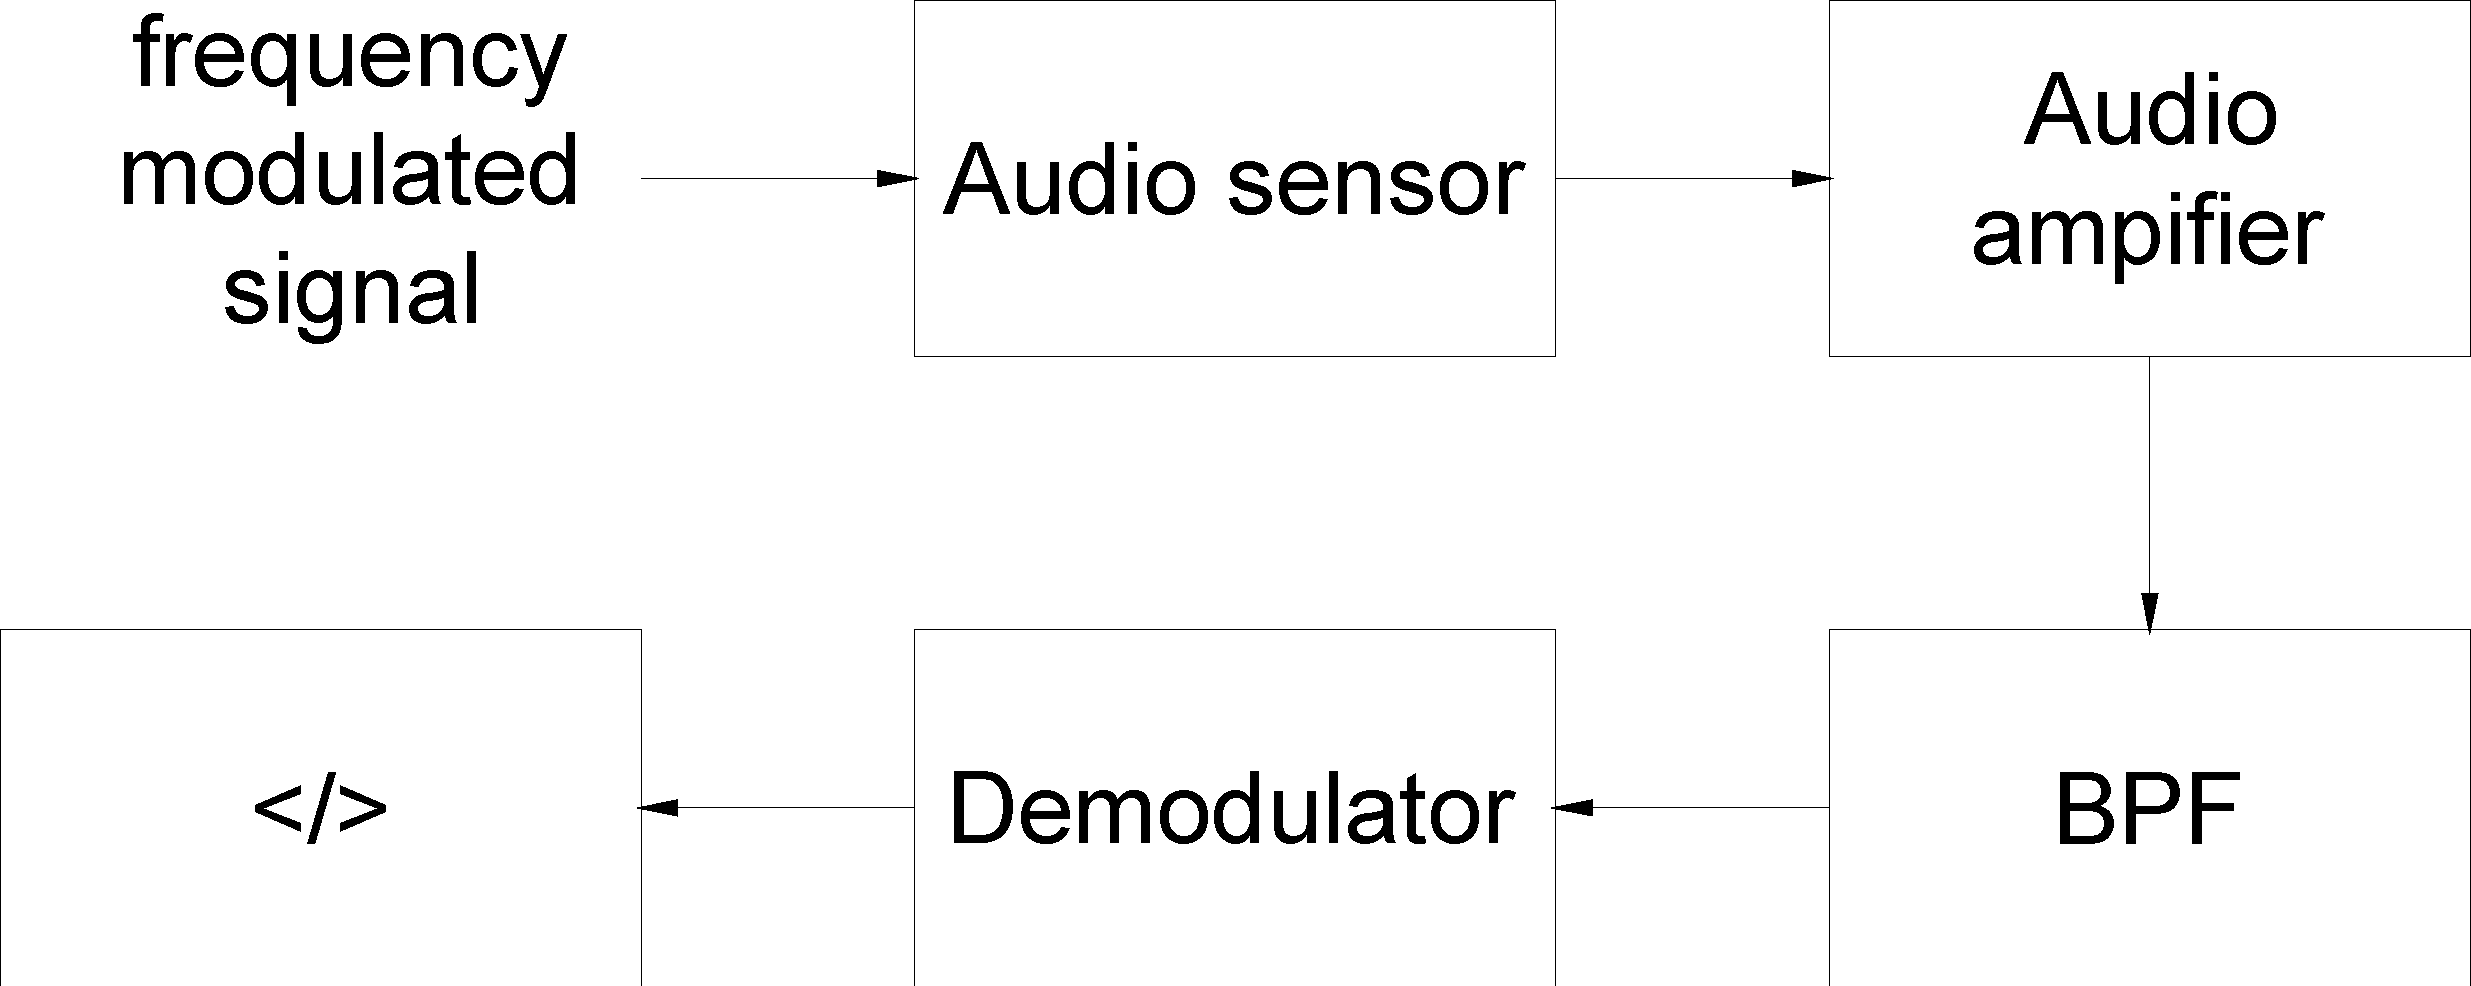
\includegraphics[width=0.8\textwidth]{demodulator.pdf}
  \caption{Demodulator}
  \label{demodulator}
\end{figure}

\subsection{Wireless communication} 

The specifications of the wireless communication are  discussed in our framework, but will be shortly summarized. 

\begin{table}[H]
\centering
\caption{Wireless communication module}
\label{wirelesscommunication}
\begin{tabular}{|l|l|}
\hline
Module    & Wireless communication module \\ \hline
Input  & \begin{tabular}[c]{@{}l@{}}Communication with the system\\ Communication with the other robots in the swarm          
\end{tabular}   \\ \hline
Output & \begin{tabular}[c]{@{}l@{}}Communication with the system\\ Communication with the other robots in the swarm         
\end{tabular}   \\ \hline
Functions   & \begin{tabular}[c]{@{}l@{}}establishes the communication between the modules swarm \\ Obtains information regarding the distance between the different robots\end{tabular}            \\ \hline
\end{tabular}
\end{table}

To communicate between different units a communication network should
be set up with a common protocol . In addition, the protocol must be able to
provide additional information such as localization. See Table \ref{wirelesscommunication}. 

\subsubsection{Central control unit}

The central control unit handles all communication between the various modules that are present on the robot. See Table \ref{control}

\begin{table}[H]
\centering
\caption{Central control unit}
\label{control}
\begin{tabular}{|l|l|}
\hline
Module    & Central control unit \\ \hline
Input  & All information from the system  \\ \hline
Output & All control of the modules in the robot \\ \hline
Functions  & All the communication comes together and controls the inputs and outputs            \\ \hline
\end{tabular}
\end{table}




\section{Design}
Now that specifications of the functional blocks are defined, a implementation for these blocks will be found, using the information from the research phase. Just like section Functional specifications every block will be discussed independently. How all of the functional blocks fit together will be discussed in the section for the central processing unit.


\subsection{Short range localization sensor}
The short range localization consist of multiple smaller parts: Acoustic actuator/sensor, modulation/demodulation, distance measurement, and angle algorithm. The code shown in this section is written for a Xmega256a4u.

\subsubsection{Acoustic actuator sensor}
As stated earlier a short range localization will be implemented using acoustic wave signals. The sensor will be implemented using microphones and an actuator will be implemented using a speaker. 

For Trigonometry angle determination the module must atleast poses three microphones spread in a triangle where all sides have the same distance as shown in figure \ref{module}.

For the distance between the different microphones a length of 10 cm is chosen because with the velocity propagation of sound being 343.2 m/s (at 20\degree C Celsius) and the underlying distance between the microphones being 10 cm using an 32 MHz micro-controller should grant enough overhead time to process the three different times being detected by the microphones. 

\begin{figure}[H]
\centering
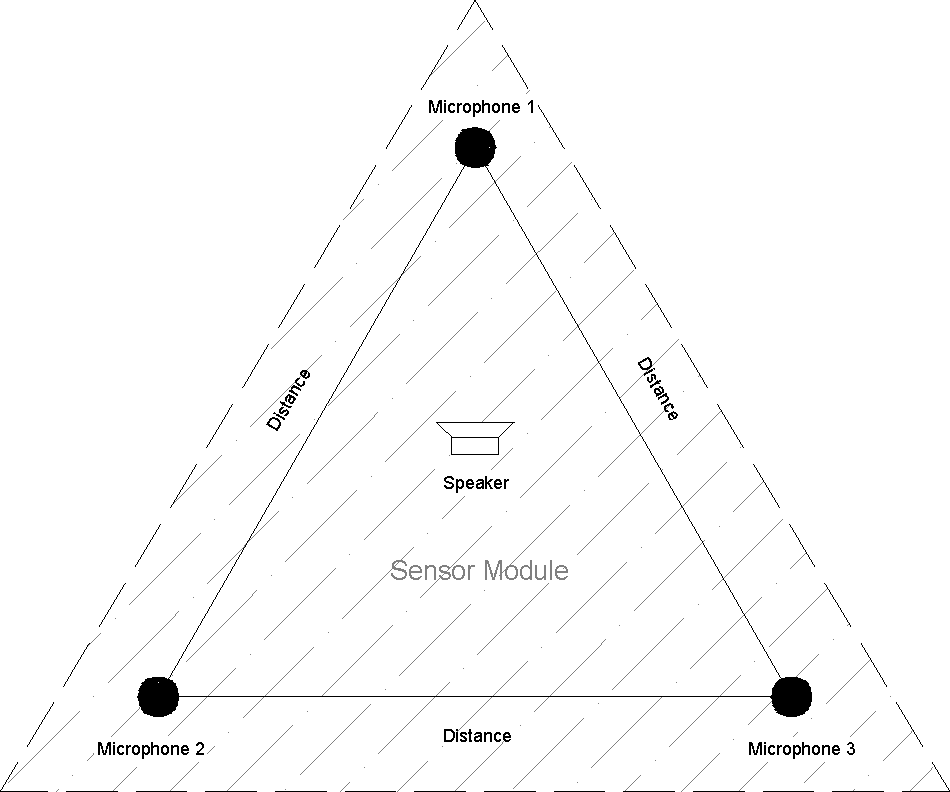
\includegraphics[width=1\textwidth]{Module.pdf}
\caption{Localization Module}
\label{module}
\end{figure}

The acoustic signal is send by a speaker facing upward. A metal plate is placed a 3 mm above the speaker, tests during the research phase showed this greatly improved the omnidirectional spread of the signal. The signal that's send it chosen to have a frequency of 3,8 kHz which has the best omnidirectional and range properties (section 4 of the research document).


The signal received by the microphone, translates in just a few millivolts. This signal is amplified 48 times. Then the signal is fed into the ADC of the Xmega256a4u. The sender code and receiver code will now be discussed in detail.\\\\

\subsubsection{Acoustic sender}
The signal is being generated within a micro-controller and sent to the speaker using a digital to analog converter. This signal is first being amplified to make sure it is loud enough. The block diagram for modulating this signal is shown in figure \ref{fig:modulatorblock}. The signal is set at 3764 Hz, it
consists of an array using 50 samples per period. The sender will send out a series of 10 "beeps", every beep consists of 1250 samples of the 3764 Hz signal. For every beep the sending  module sends a interrupt signal to the receivers. The mean is taken of the array samples of the five sampled signals. The code for the acoustic sender is shown below.

\begin{figure}[H]
    \centering
    \includegraphics[width=0.65\textwidth]{Modulator.pdf}
    \caption{Modulator block diagram}
    \label{fig:modulatorblock}
\end{figure}

\lstinputlisting[firstline=22,lastline=88,
label=code:sendercode, 
caption= Acoustic sender code]
{./code/mainsinegen.c}
In the next sections the workings of the receiving end will be explained.

\subsubsection{Acoustic receiver}
The signal send by the acoustic sender is received by the microphone of the receiving modules. As discussed in the research section, a simple version of cross-correlation is used to determine the TOF (time of flight) of the acoustic signal. The receiving micro-controller has a copy of the array that is used to create the signal in the sending micro-controller.
When the receiver, receives an interrupt from the sender it will start to sample data from the ADC that's connected to the microphone. The sampling time is 50 times per period, this is exactly the same as the sending side. Ten individual beeps are sampled. The mean is taken from the five individual samples before the cross-correlation algorithm is performed to determine the distance. For further explanation on the simplified version of cross correlation used see section  \ref{sec:simplecross}. A Block representation is given of the receiving side shown in figure\label{fig:demodulatorblock}.



 \begin{figure}[h]
     \centering
     \includegraphics[width=1\textwidth]{Blokschemareceive.pdf}
     \caption{Block representation of the receiving side}
     \label{fig:demodulatorblock}
 \end{figure}

The distance is derived from the time it takes the acoustic signal to travel from module A to module B. 
Suppose that module A is about to send its signal. Just before it starts sending the acoustic signal, it sends a message over the radio communication, which is almost instant compared to the speed of the sound waves. Module B starts its timer and wait for the signal to arrive. The distance can now be derived multiplying the speed of sound with the measured time. The state diagram for the distance measurement is shown in \ref{fig:distancemk}.

\begin{figure}[H]
    \centering
    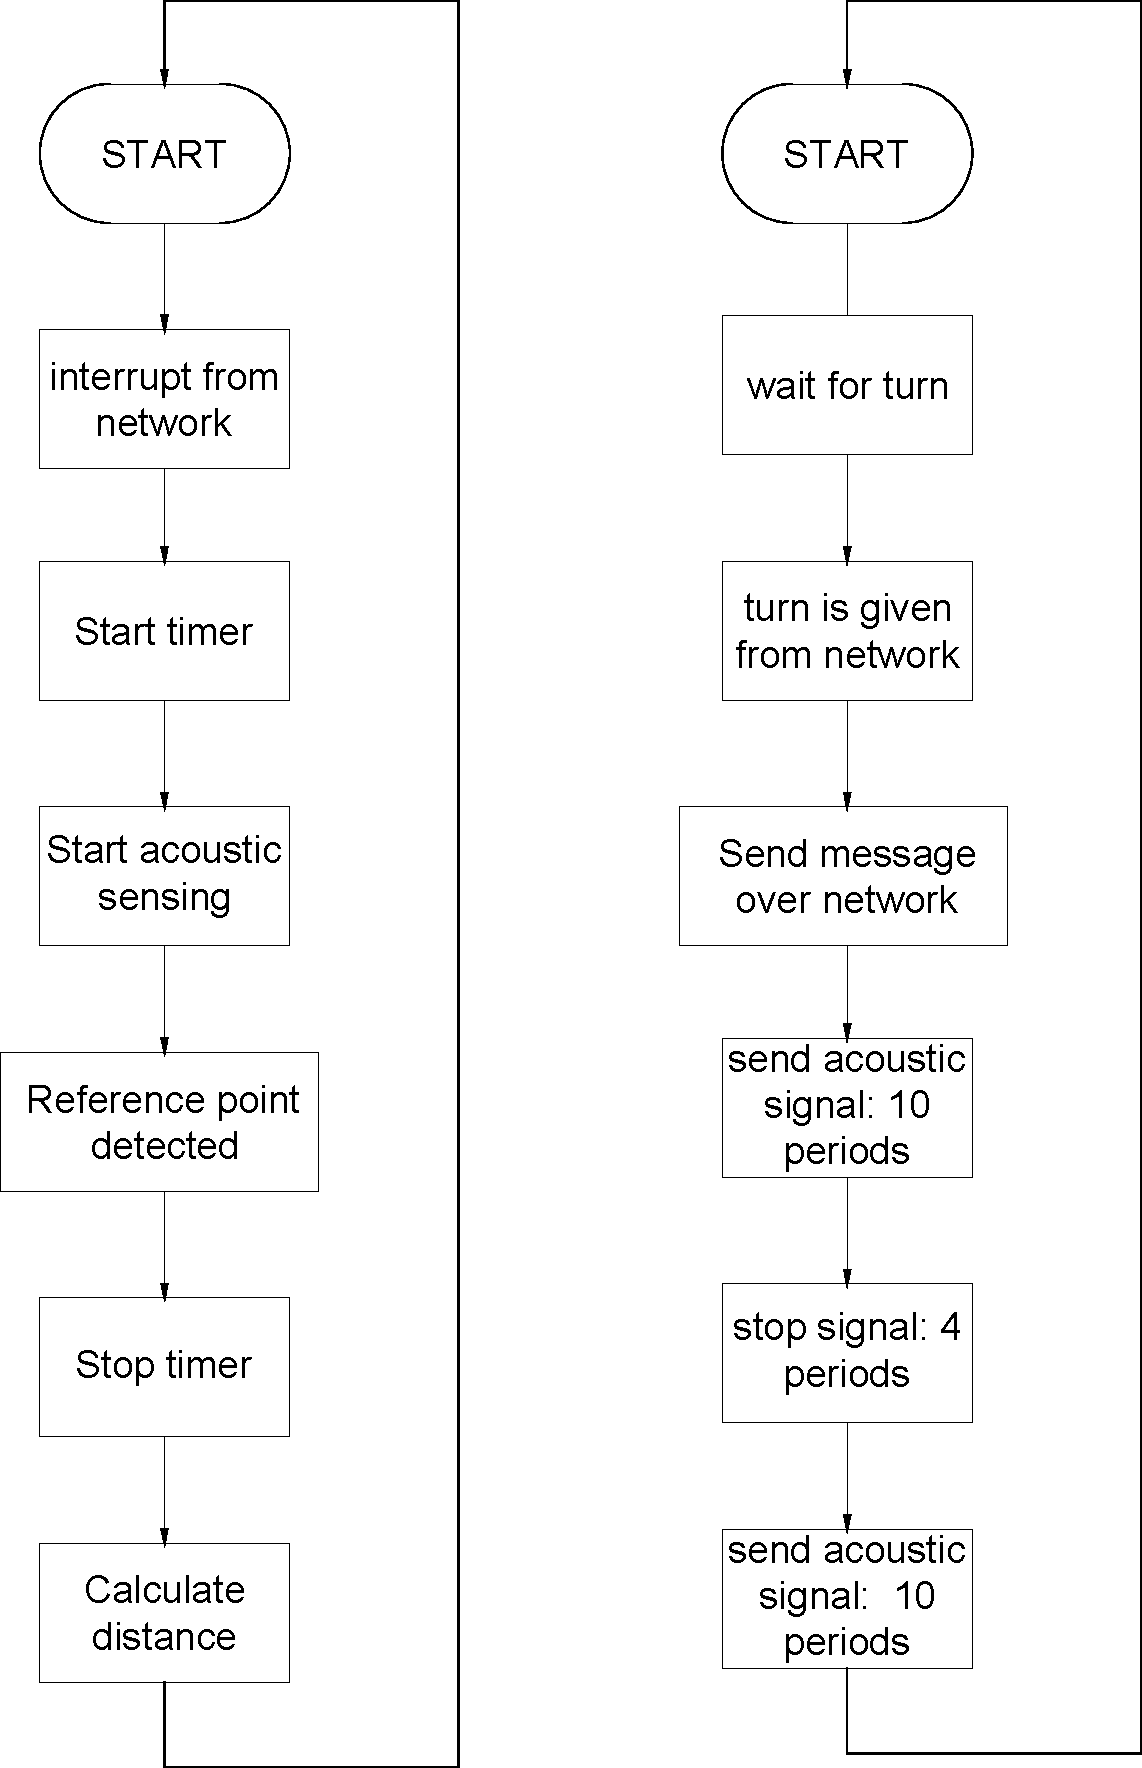
\includegraphics[width=0.65\textwidth]{distancem.pdf}
    \caption{State diagrams for the distance measurement. The diagram on the right is for the receiving side, and the left diagram is for the sending side.}
    \label{fig:distancemk}
\end{figure}

This state diagram is translated in C code shown in \ref{code:receivingcode}. The correlation function can be found in the research section.

 \lstinputlisting[firstline=13,lastline=78,
label=code:receivingcode, 
caption= Acoustic receiver and correlation code]
{./code/maincorrelation.c}


\subsubsection{Angle measurement and relative location}
The Swarming module has three microphones placed with known distances between them. The relative angle is derived from the time measured with each microphone, and the distance between the microphones. In section 3.2 there's more information on how the algorithms needed. The following algorithm shows pseudo-code how the angle and relative location is derived from the three measured distances.
No implementation of this pseude-code was achieved during this project. A reliable distance measurement is needed to derive the angle using this method. Small deviations in the distance can cause far bigger deviations in the angle, due to the relatively small distance between the microphones.
The distance measurement achieved during this project, will still need further tweaking before it can be used for localization.
\lstinputlisting[firstline=1,lastline=40,label=code:locationalgo,caption=Algorithm to derive the relative location]{./code/Location_algorithm.c}

\subsection{Swarm communication implementation}
During the research, we came across some plug and play wireless swarm communication implementations. One of these implementations is the SwarmBEE LE module from Nanotron. The SwarmBEE LE module meets the given network criteria and most of the recommendations. The module uses a radio frequency 2,4 GHz signal as a communication channel. The module is not only a communication module, but can also be used to determine relative distances to each swarming module. It also has a API with predefined functions which can be used to set up the wireless network.



\subsubsection{Central operating unit}

In Table \ref{cou} the basic specifications of the AtXmega128A4U are shown. This is the microcontroller used in as the central operating unit. The microcontroller from Atmel complies with all the specifications. There are also newer micro controllers available, but are not yet implemented for this project, since the older versions can handle the workload and work fine. There are two $I^2$C connections available on the microcontroller which are needed to connect the module to the robot. Also the multiple ADC and DAC connections can come in handy if any sensors or actuators need to be added to the module. Overall the AtXmega128A4U fits all the specification that are required, and there is room to expand the functionality when it is necessary. An overview of all the specification can be found on the website of Atmel.


\begin{table}[]
\centering
\caption{Central operating unit}
\label{cou}
\begin{tabular}{|l|l|}
\hline
\textbf{Parameter}			& \textbf{Value} \\ \hline
Flash (kBytes):             & 128 kBytes \\ \hline
Pin Count:                  & 44         \\ \hline
Max. Operating Freq. (MHz): & 32 MHz     \\ \hline
CPU:                        & 8-bit AVR  \\ \hline
Max I/O pins:               & 34         \\ \hline
USB Interface:              & Device     \\ \hline
SPI:                        & 7          \\ \hline
TWI (I2C):                  & 2          \\ \hline
UART:                       & 5          \\ \hline
ADC Channels:               & 12         \\ \hline
ADC Resolution (bits):      & 12         \\ \hline
ADC Speed (ksps):           & 2000       \\ \hline
DAC Channels:               & 2          \\ \hline
SRAM (kBytes):              & 8          \\ \hline
EEPROM (Bytes)              & 2048       \\ \hline
Operating Voltage (Vcc):    & 1.6 to 3.6 \\ \hline
\end{tabular}
\end{table}

The Central operating unit handles multiple functions to make the group of robots a swarm. Those functions will be explained in this section.
There are four major functions that are implemented in the microcontroller. Controlling communication that goes in and out, storage and maintain data, calculating the population of the swarm and send and receive message that are used for localization. The communication will be mainly about the communication with the Swarmbee module. The connection to the robot is just as important but will not be thoroughly discussed in this document. First of all we will discuss the implementation of the communication.

\subsubsection{Communication}

The central operating unit needs to send request and receive data from the Swarmbee module. This information is transmitted using the UART protocol. The communication is mainly used for sending API commands to the Swarmbee module. The UART connecting uses a baudrate of 115200 bps since this is the transmission speed of the Swarmbee module. The Xmega uses two pins, RX (PC2), TX PC3) to achieve a wired connection with the Swarmbee. The module needs to be able to communicate with a robot platform. To communicate with this platform the module uses $I^2$C communication. This should be standard for every robot, so that the module can easily be placed on any type of robot platform.
For debugging pin C7 en C8 are reserved. The debugging connecting can be established with a terminal such as Putty.



\begin{figure}[H]
   \centering
   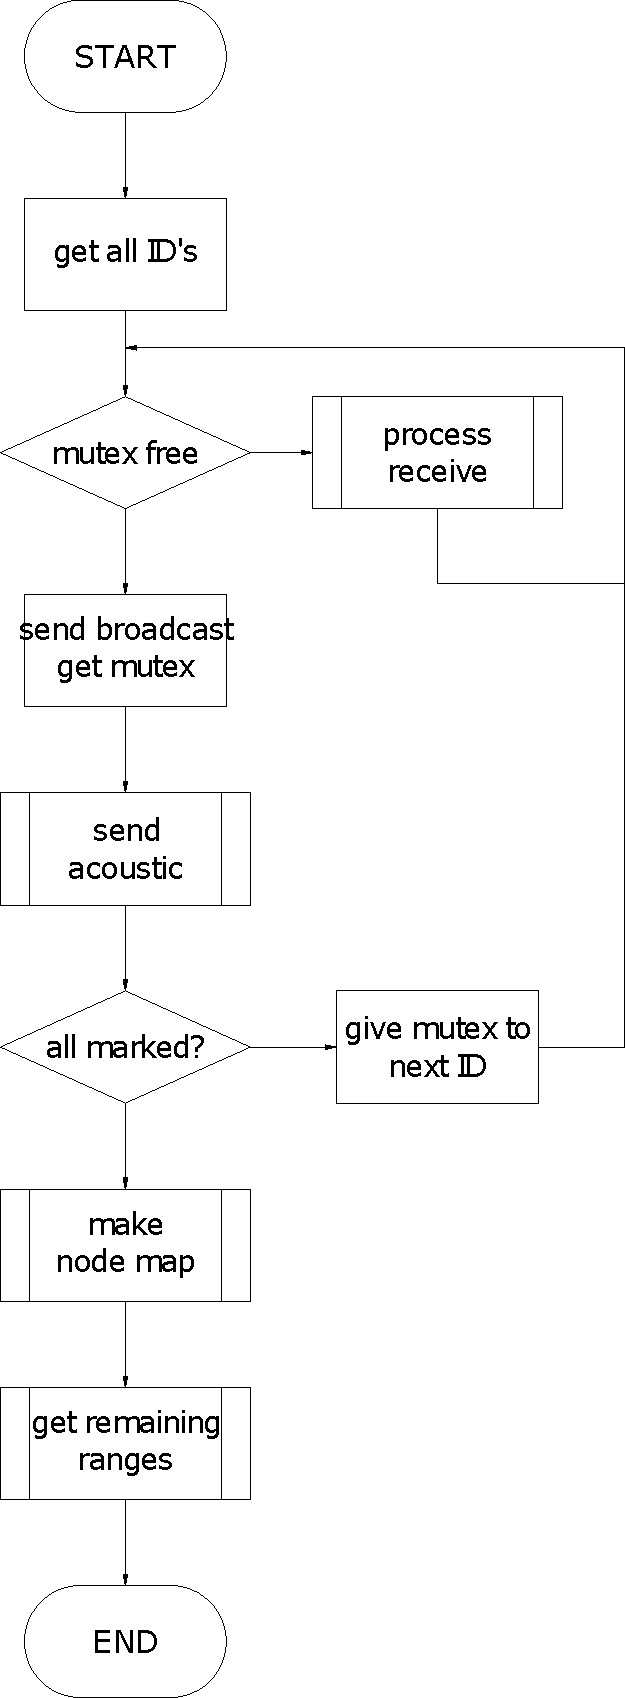
\includegraphics[scale=0.5]{mainal.pdf}
   \caption{main algorithm for updating the swarm population including range requests}
   \label{fig:mainal}
\end{figure}


\subsubsection{Swarm population}
To update the swarm population all modules need to receive the ID's from other modules in range of the Swarmbee module. This is the first step in the flowchart of the main algorithm shown in figure  \ref{fig:mainal}. The swarmbee automatically assigns a unique ID to all nodes. A list of all nodes and the corresponding ranges can be requested from the swarm by a API broadcast message "*RRN". This broadcast message can be requested at a certain interval which depends on the demand of this information. The broadcast interval can be set via a command; "sbiv 1000", where sbiv stands for "set broadcast interval" and the time is set at 1000ms, or 1 second. When the swarmbee receives a ranging request its response will look somewhat like this:

\lstinputlisting[firstline=1,lastline=1,label=code:rrn,caption=]{./code/swarmbeeex.c}

Where the first two hexadecimal values represent the source ID (sending module), and the destination ID (receiving module). This is followed up by an error code and the range relative in centimetres to the destination node. The end of the message contains a custom value which can be set by a "notification configuration"-request. For example, this value can represent different sensor values like; x,y,z acceleration, the measured RSSI value or the current battery level.

To fill the population list with including ranges first, the module needs to know its own ID. This can be received by a command, "GNID", or "get node ID". A volatile variable "myid" will be set to this string.

Now that the node knows its own id the population list can be filled with information. A frame in the list will look like this:

\begin{figure}[H]
    \centering
    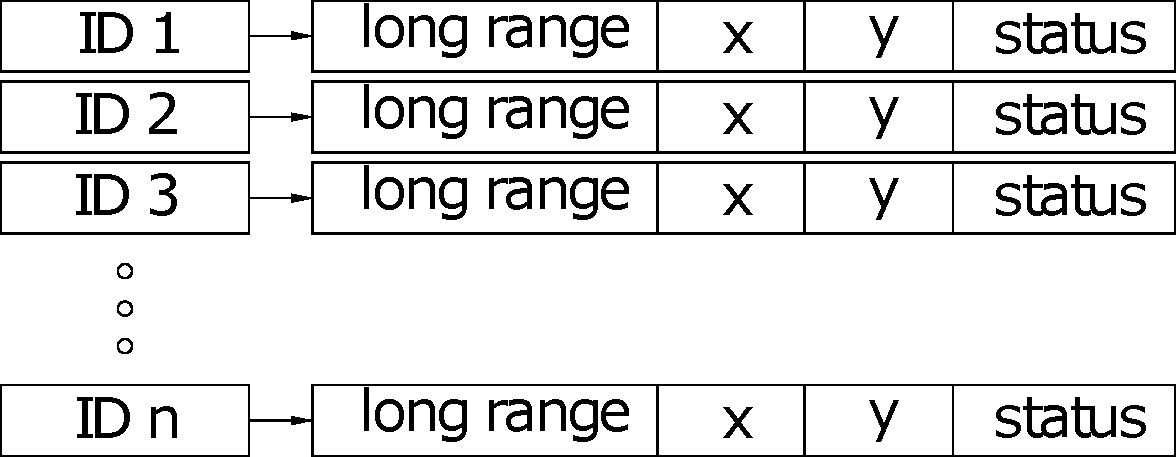
\includegraphics[scale=0.45]{popframe.pdf}
    \caption{One population list frame}
    \label{fig:frame}
 \end{figure}

Where the ID and the longrange can be received from the swarmbee module, the x and y coordinates are from the acoustic sensing algorithm and the status is set by the main algorithm.

The following code describes how this function will be executed.
\lstinputlisting[firstline=1,lastline=41,label=code:fillpop,caption=]{./code/fillpop.c}

This function will be executed when the received message is a ranging request notification, because this is the message that will be the argument of this function. At line 16 a while loop starts filling: srcid, destid and distance with the corresponding information from the ranging request notification. A comma indicates that a new value starts. At line 34 and 37 the received id's are compared to its own id so that the right id will be set with the range. The id's and longranges are now filled in the population list.  

\subsubsection{Acoustic sensing send/ receive}
After all node ID's are known the first swarm unit in queue will get the mutual exclusion to be the only sender in the acoustic ranging process, it will enter the "send acoustic"-process, figure \ref{fig:sendre}.1. since only one member can be the sending module the rest of the swarm will enter the "process receive" algorithm, figure \ref{fig:sendre}.2. When a node is done sending it will set a mark and send a broadcast to the rest of swarm. The status bit in the frame (\ref{fig:frame}) will be set as one, now all members know that this ID is done. The "order"-function(pseudocode) will keep checking who is the lowest in queue. When all id's status bits are marked the complete algorithm is completed.

\lstinputlisting[firstline=1,lastline=10,label=code:order,caption=]{./code/order.c}

When the swarm module is in sending mode it will send out a sound signal and retrieve the ranging results form the receiving modules one by one. The receiving modules will start the localization algorithm when a request from the sender is received. When there is no result a node will be marked as "out of range". When a sender retrieved all ranges this node gets marked as 'done'. The main algorithm, figure \ref{fig:mainal}, will now give the mutex to the next swarm member until all units are marked. When all nodes are marked, each module will create its own node map. When there are any missing ranges these gaps will be filled by the (long) ranges received by the swarm bee in the ranging request broadcast message.

\begin{figure}[H]
   \centering
   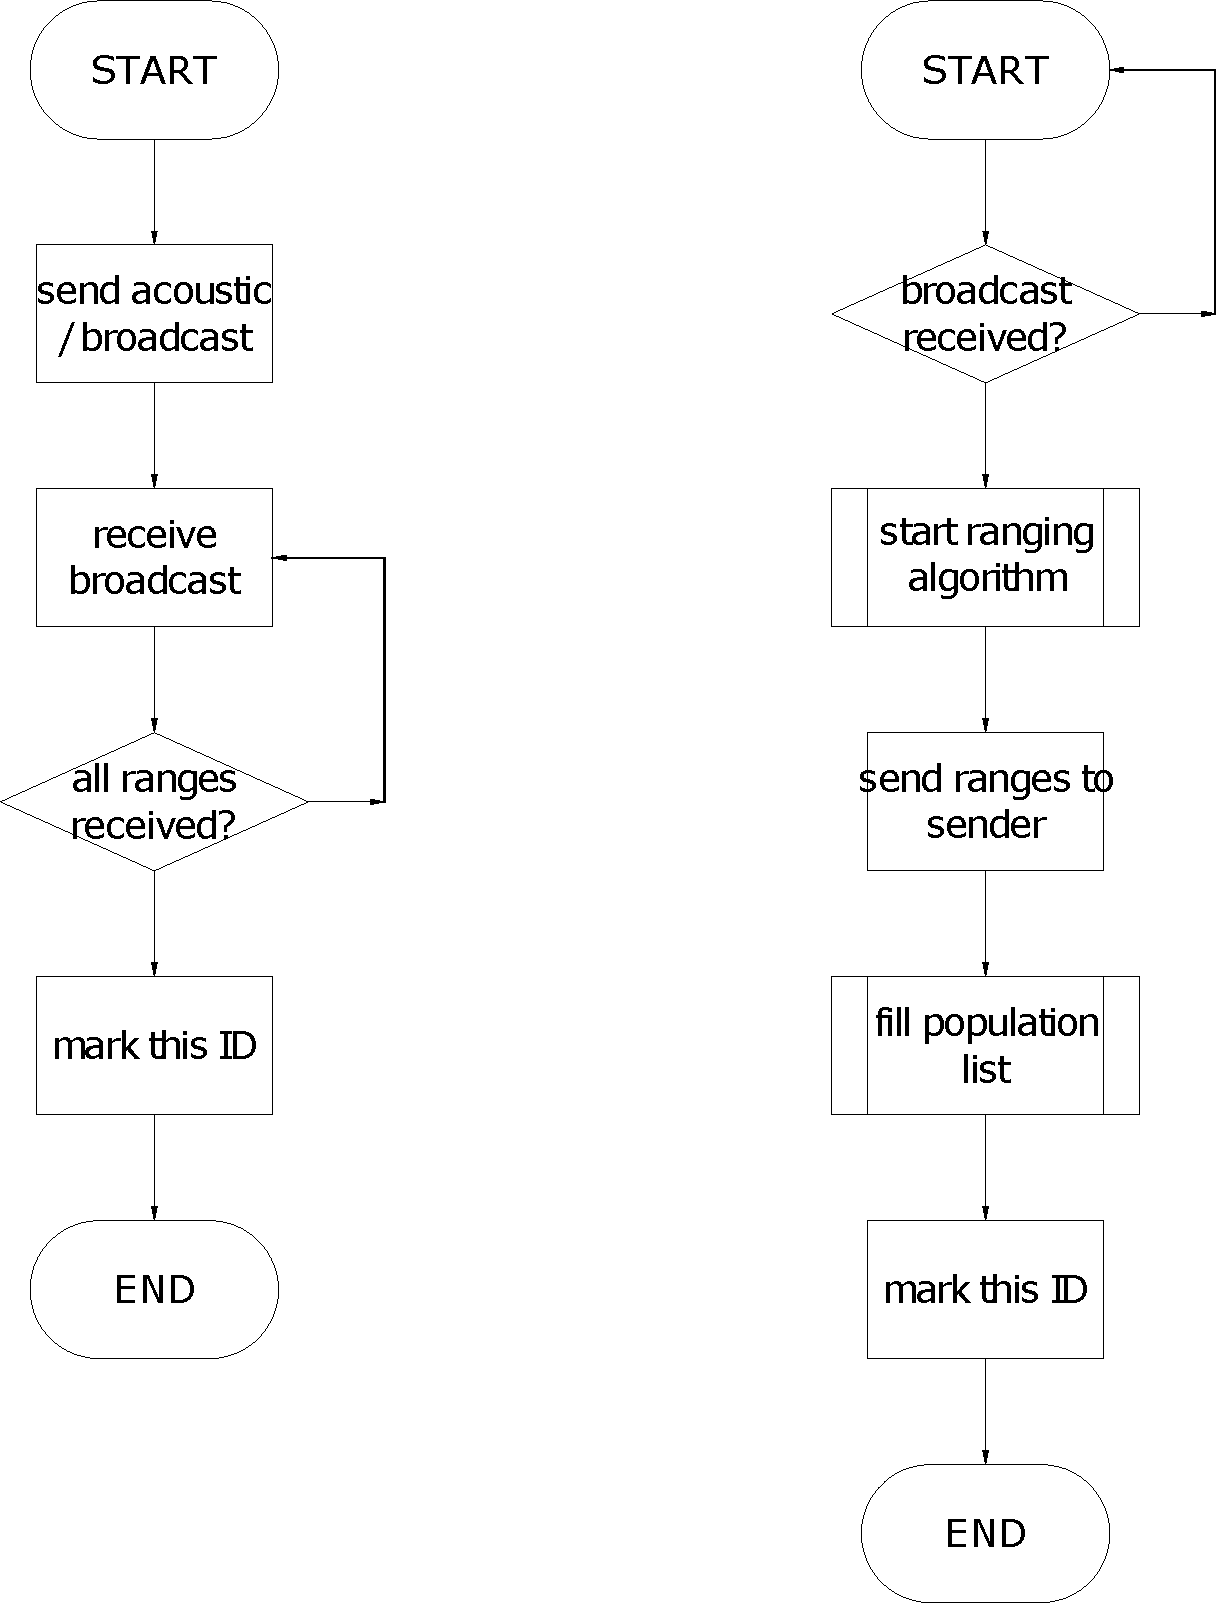
\includegraphics[width=\textwidth]{sendre.pdf}
   \caption{1:"send acoustic" when the swarm module is in sensing state 2:"process receive", when the swarm module is in receiving state}
   \label{fig:sendre}
\end{figure}

\lstinputlisting[firstline=1,lastline=26,label=code:sender,caption=]{./code/sender.c}
\lstinputlisting[firstline=1,lastline=21,label=code:receiver,caption=]{./code/receiver.c}

The communication module uses two UART connection. One for the communication with the swarmbee module and one for debug purposes. Two functions have been made to keep those data channels separated from eachother.

The validatemessage compares the received message with a defined type of message length. The type of messsage is defined by another function, "DetermineCommandType". This function separates the first characters of the message (the command characters) from the rest. Based on the first separated command characters it executes the intented function.
\lstinputlisting[firstline=24,lastline=44,label=code:validatemessage,caption=Validates the integrity of the received message.]{./code/transceive.c}
\lstinputlisting[firstline=141,lastline=177,label=code:determinemessage,caption=Determines the meaning of the message.]{./code/transceive.c}


The translateMessage function receives byte for byte from the swarmbee modules and forms the intended messages.
\lstinputlisting[firstline=187,lastline=203,label=code:determinemessage,caption=Translates the received message. Converts characters to a single string]{./code/transceive.c}



\subsubsection{Population list}
As the specifications stated, the swarm population must be dynamic. This means that the gathered data must be stored in a dynamic list. Just as the other parts of the code, this is implemented in C code.

The dynamic list is based on the linked list principle, where the next item is linked to the previous item. Each 'item' consists of a one dimensional array with string values. This principle is equivalent to an two dimensional array, but makes it a lot more complex. 

A structure 'node' is defined and consits of a pointer to next node and the data located at the current item adress. The first item that gets inserted starts at the head (beginning of the adress range).

\lstinputlisting[firstline=18,lastline=21,label=code:structnode,caption=Linked list node structure.]{./code/list.h}

Not every function writen is used in the final code for the swarmbee. For future use and the development and debug purposes, these functions are still usefull. The following enumeration summarizes the purpose of each function:
\begin{itemize}
\setlength\itemsep{0em}
    \item SizeOfList - Amount of modules in the list
    \item PrintHeaderList - Used for debug purposes
    \item PrintList - Used for debug purposes
    \item AppendList - Inserts a data array row to the end of the list
    \item InsertList - Inserts a data array row at the beginning of the list
    \item PopListByNumber - Reads a data array row at the given index number and removes it afterwards
    \item PopListByValue - Reads a data array row with the given first value of the current row and removes it afterwards
    \item PopList - Reads a data array row at the beginning of the list and removes it afterwards
    \item ViewListByNumber - Reads the data array row at the given index number
\end{itemize}

The following is the implementation of the insert and append function. In the final code only the insert function is implemented. This is done to create a first in first out buffer, this is explained later with the pop functions.

\lstinputlisting[firstline=64,lastline=74,label=code:appendlist,caption=Inserts a data array row to the end of the list]{./code/list.c}

\lstinputlisting[firstline=87,lastline=99,label=code:insertlist,caption=Inserts a data array row at the beginning of the list]{./code/list.c}

The code for the pop functions can be found in the following three code snippets. The pop by number is implemented because of the chronologic order. It retrieves the total amount of rows in the list and begins to pop at the last and finishes at the first row.

\lstinputlisting[firstline=113,lastline=127,label=code:poplist,caption=Reads a data array row at the beginning of the list and removes it afterwards]{./code/list.c}
\lstinputlisting[firstline=141,lastline=165,label=code:poplistbynumber,caption=Reads a data array row at the given index number and removes it afterwards]{./code/list.c}
\lstinputlisting[firstline=178,lastline=200,label=code:poplistbyvalue,caption=Reads a data array row with the given first value of the current row and removes it afterwards]{./code/list.c}
\lstinputlisting[firstline=209,lastline=218,label=code:sizeoflist,caption=Amount of modules in the list]{./code/list.c}


An example of the debug interface output. There is not data (displayed with x's) in the this example. Each 'Data[]' represents an value for example, the first one is the node ID.
\lstinputlisting[firstline=1,lastline=7,label=code:populationlist,caption=Example of the population list with x's at the place of swarm data.]{./code/populationlist.text}



\subsubsection{Wireless communication}

For the wireless communication module the most important function is that it can transmit information over atleast 100 meters. Since the specification states that the swarm must be detected within this range. The speed of the communication is not defined yet, but needs to be fast enough to handle all the messages. We estimated the speed that is necessary to handle all communication. We estimated that the maximum size of a message is 1kBytes. Since the long distance communication had an update frequency of 1Hz, the minimum communication speed that is required is 8kpbs. The Swarmbee LE module will be used for the wireless communication. The Swarmbee LE module will be used for the wireless communication. It uses the ISM band, 2.4 GHz to transmit and receive the data. The maximum range of the module relies on the environment in which it is used. Under ideal conditions the Swarmbee can reach a distance of 1200 meters. It depends on how many obstacles, reflections and interference there is to disturb the signal. An experiment from Nanotron showed that until a range of 150 meters the ranging success rate is about 100\% with a transmission speed of 155 kbps. Experiments we have done ourself show that the antenna on the device does not respond very well inside a building. Test outdoors should still be done, but there is a possibility that an external antenna is needed to reach these distances. The actual speed is also not tested yet, but could be done in the future. Transmitting data between the swarm modules can be configured with a speed of 250 Kbps or 1 Mbps. Tests will show if this will be enough. This module fits all the specifications and is suitable for the use of wireless communication.

\begin{table}[h]
\centering
\caption{Swarmbee LE module} 
\label{SwarmbeeLE}
\resizebox{\textwidth}{!}{%
\begin{tabular}{|ll|}
\hline
\multicolumn{1}{|l|}{\textbf{Parameter}}                                                                                                 & \textbf{Value}                                                                                                                 \\ \hline
\multicolumn{1}{|l|}{Frequency range}                                                                                                    & ISM band 2.4 GHz (2.4 - 2.4835 GHz)                                                                                            \\ \hline
\multicolumn{1}{|l|}{Modulation}                                                                                                         & Chirp Spread Spectrum (CSS)                                                                                                    \\ \hline
\multicolumn{1}{|l|}{Transmission modes}                                                                                                 & \begin{tabular}[c]{@{}l@{}}80 MHz, 1 Mbps or 250 Kbps\\ (80/1 or 80/4 mode)\end{tabular}                                       \\ \hline
\multicolumn{1}{|l|}{TOA capture accuracy}                                                                                               & \textless 1 ns (better than 30 cm)                                                                                             \\ \hline
\multicolumn{1}{|l|}{Typical air time per ranging cycle}                                                                                 & 1.8 ms                                                                                                                         \\ \hline
\multicolumn{1}{|l|}{RF output power}                                                                                                    & configurable - 22 t0 16 dBm                                                                                                    \\ \hline
\multicolumn{1}{|l|}{RF sensitivity}                                                                                                     & \begin{tabular}[c]{@{}l@{}}-89 dBm typ. @80/1 mode\\ -95 dBm typ. @80/4 mode\end{tabular}                                      \\ \hline
\multicolumn{1}{|l|}{RF interface}                                                                                                       & 50 Ohm RF port (for external antenna)                                                                                          \\ \hline
\multicolumn{1}{|l|}{Host interface (UART)}                                                                                              & 500bps $\sim$ 2 Mbps                                                                                                           \\ \hline
\multicolumn{1}{|l|}{Power supply}                                                                                                       & 3 - 5.5 V                                                                                                                      \\ \hline
\multicolumn{1}{|l|}{Max. supply voltage ripple}                                                                                         & 20 mVpp                                                                                                                        \\ \hline
\multicolumn{1}{|l|}{Active power consumption*}                                                                                          & 120 mA during transmission, 60 mA during receive in 80/1 mode                                                                  \\ \hline
\multicolumn{1}{|l|}{Power consumption in sleep mode*}                                                                                   & 5.5 mA (transceiver disabled, all peripherals on)                                                                              \\ \hline
\multicolumn{1}{|l|}{Power consumption in snooze mode*}                                                                                  & 4.5 \si{micro}A (transceiver disabled, all peripherals off, wake-up by timer)                                                           \\ \hline
\multicolumn{1}{|l|}{Power consumption in nap mode**}                                                                                    & \begin{tabular}[c]{@{}l@{}}4.5 $\sim$ 600 \si{micro}A (transceiver disabled, all peripherals off, wake-up by \\ interrupt)\end{tabular} \\ \hline
\multicolumn{1}{|l|}{Power consumption in deep-sleep mode*}                                                                              & \textless 1 \si{micro}A (device completely disabled)                                                                                    \\ \hline
\multicolumn{1}{|l|}{Operating temperature range}                                                                                        & -30 - 85 $^{\circ}$C                                                                                                                    \\ \hline
\multicolumn{1}{|l|}{Dimensions}                                                                                                         & 40 mm x 24 mm x 3.5 mm                                                                                                         \\ \hline
\multicolumn{1}{|l|}{Weight}                                                                                                             & 7 g                                                                                                                            \\ \hline
\begin{tabular}[c]{@{}l@{}}*Power consumption in all modes is \\ measured at 20$^{\circ}$C, 3.3 V.\end{tabular}                                   &                                                                                                                                \\ \hline
\begin{tabular}[c]{@{}l@{}}**Power consumption in nap mode \\ depends  on interrupt sources (GPIO \\ pins or MEMS or both).\end{tabular} &                                                                                                                                \\ \hline
\end{tabular}%
}
\end{table}

\newpage

\section{Results and Discussion}
It is essential that the communication is reliable and can handle the workload. If the communication is not working properly the whole system will fail. In the previous sections all the design choices are written down and explained. The result is a working swarm module that can be controlled in the way you want the swarm to work. All incoming and outgoing messages are handled reliable and can be easily accessed. The communication uses UART to handle internal communication with micro-controller and uses $I^2$C to handle the communication to the platform where the module will be installed. An added feature is that the communication now keeps track of the population. This was not a feature on the Swarmbee yet, but now the tracking is accurate and reliable. The Swarmbee modules are not tested to work like an actual swarm yet, but the only reason is that because there is not any swarm objective implemented. If the instructions are send to the swarm modules these can be send to the central operating unit of the robot where the robot can give a fitting response. The module can also determine the distance between each swarming module. This should work fine but there are some minor issues , which can be worked on in the future. The test with these feature where mainly done inside, but should work fine outdoors. Also the standard antenna is used, but a more powerful antenna could be easily implemented.

Three implementations of relative localisation are proposed. Two of which did not meet the expected specifications. The first method using the analog PLL was supported by thorough research but the theory did not meet the experiments in practice. The problem was found to be the comparator circuit which would cause differences in the delay caused by the circuit. This made the circuit unfit for our cause. It was then decided to use digital signal processing to find the reference point in the acoustic signal. This first method used a comparator of the micro-controllers ADC. Without noise this method worked well enough to measure the signals frequency. But with just small amounts of noise like people talking the frequency could not be measured. Attempts were made to reduce the noise using a small banded filter but this did not help enough to make the measurements constant. The third attempt is were the project stands now and uses convolution to determine the time delay in the signal. This research is still in the early stages, results might be added in a later version of the document.

\section{Conclusion}
The conclusion is divided into two subsections, Swarm communication and Relative localization. As described in project method the V-model was used to give the project structure. As part of the V-model specifications defined in every phase should be tested. For this the qualification document is created and will be included in the same folder as this document. However no actual testing could be done because there is no finished product to test.

\subsection{Swarm communication}
The following research questions for swarming communication were drafted:
   
    \begin{itemize}
        \item "What software protocol should be used?"
        \item "How do the units communicate within the swarm?"
        \item "What is the minimal required communication speed?"
        \item "What hardware is needed to implement the communication?"
    \end{itemize}
    
During this project all of the questions were answered. A unit can communiaite with the swarming via the Central operating unit, which in turn communicates with the Swarmbee module that maintains the swarm network. The Swarmbee module is used to set up the swarm network. This uses a 2,4Ghz protocol. The software used determine the swarm population is self written and explained in the design section of this document. The minimal required speed is estimated around 8kbps, which is easily reached by the Swarmbee module. With all the questions answered the swarm communication is mostly done. Practice tests still need to determine whether or not the system works properly.

\subsection{relative localization} 
The important research questions for the relative localization are:

    \begin{itemize}
        \item "What is the definition of swarming?"
        \item "How do robots in the swarm know their location?"
    \end{itemize}

Swarming was first defined to determine the specifications for the relative localization. It was found that the angle measurement did not have to be real precise for the localization to be useful for the swarm. Algorithms were drafted to determine the location of other units using three microphones on predefines locations on the module itself. To implement actual localization, a reliable distance measurement first had to be implemented. A distance measurement was implemented that met the specifications to a distance of 1,5 meter. However due to many setbacks while trying to implement this,  no time was left to implement a way to measure the relative angle.


\section{Recommendations}
The progress of this project is not as far as we had hoped for, and there are many things that can be improved to make the module as complete as possible. As far for the communication part, most of the functions are completed, except for a few. If there was more time we would have tried an implementation for the swarm to test if the modules would really work in a swarm, and then swarming behaviour could be confirmed. This is something that should be done in the next phase of this project. As said before the communication with the acoustic sensor is not established yet. This is a vital part for the module in order to make it work as a whole. This is definitely a must in a next phase, but it could not fit our timetable in this phase, and we had prioritize our tasks. The distance determination of the Swarmbee module is not tested thoroughly and is critical if you want a reliable Swarm. If the distances are not correct, it could have sever consequences. There are still some tasks that need to be done. The tasks just mentioned should be done first in a next stage of this project.

We still recommend using acoustic signals to determine the distance. We found that analog solutions cause to many deviations in time to create a usable implementation. Digital signal processing seems the best way to deal with the problem. The properties of the signal that was to be received are already known. Because of this we propose the use of convolution (discussed in chapter 5.3). Convolution allows for noise-heavy signals to be detected and used. 


There are a few points of interest to improve the code. These points might make the code quicker and more reliable. Two problems that were encountered with the current micro-controller, that is used for this project, are its limited memory and processing power. One method to overcome these obstacles is by adding up the values read from the ADC, this means not every read value needs its own space in the array. With the current ten measurements of 1250 samples each that would mean saving up to 16.875 bytes when using 16-bit integers in said array. Since the total data memory of the ATXMega128A3U is only 16KB this solution would save a lot of memory in the micro-controller. Using the previous solution also means the correlation-algorithm will get an average outcome from the ten measurements. A second point of interest to make the measurement more reliable while not slowing down the measuring process too much, is by using Paul Bourke's cross-correlation algorithm. But instead of using floating point calculations, which requires a lot of processing power, we recommend using fixed point calculations. The micro-controller can handle these calculations much better than floating point calculations, improving the speed drastically. Using this method it is assumed that the measurement will be more reliable. 
A determination has to be made what kind of precision is needed from the distance measurement to implement a angle measurement with a resolution of 45$\deg$.
We recommend using a simulation program like Mathlab to run the full algorithm using stored values from the ADC, to determine if the specifications can be met using this algorithm. Once this is proven the algorithm can be ported to the micro-controller. Another way to overcome the problem of the limited amount of memory is by connecting extra external memory, like an SD-card for example. The current micro-controller used has an external slot to connect an SD-card, if this can be configured the amount of data will not be a problem any more. The only thing that should be taken into account is that reading and writing to the SD-card might not be fast enough for all the variables used. When correlation does not meet the specifications the recommendation is trying to implement 'code 1' with a frequency based approach, but instead of using the analog comparator using the ADC this might make it less susceptible to noise.

\newpage






\section{References}
\bibliography{references}
\bibliographystyle{IEEEtran}





\end{document}
